%%%%%%%%%%%%%%%%%%%%%%%%%%%%%%%%%%%%%%%%%
% Arsclassica Article
% LaTeX Template
% Version 1.1 (1/8/17)
%
% This template has been downloaded from:
% http://www.LaTeXTemplates.com
%
% Original author:
% Lorenzo Pantieri (http://www.lorenzopantieri.net) with extensive modifications by:
% Vel (vel@latextemplates.com)
%
% License:
% CC BY-NC-SA 3.0 (http://creativecommons.org/licenses/by-nc-sa/3.0/)
%
%%%%%%%%%%%%%%%%%%%%%%%%%%%%%%%%%%%%%%%%%


\documentclass[
10pt, % Main document font size
a4paper, % Paper type, use 'letterpaper' for US Letter paper
oneside, % One page layout (no page indentation)
%twoside, % Two page layout (page indentation for binding and different headers)
headinclude,footinclude, % Extra spacing for the header and footer
BCOR5mm, % Binding correction
]{scrartcl}

\input{structure.tex} % Include the structure.tex file which specified the document structure and layout
\hyphenation{Fortran hy-phen-ation} % Specify custom hyphenation points in words with dashes where you would like hyphenation to occur, or alternatively, don't put any dashes in a word to stop hyphenation altogether
\usepackage{makecell}
\usepackage{xcolor}
\usepackage{fancyvrb}
\usepackage{tikz}
\usepackage{tikzscale}
\usepackage{pgfplots}
\usepackage{xcolor}
\usepackage{graphicx}
%\usepackage{algorithm}
%\usepackage{algorithmic}
\usepackage[ruled,vlined]{algorithm2e}
\usepackage{hyperref}


\usetikzlibrary{snakes,arrows,shapes}
\usetikzlibrary{arrows.meta}
\usetikzlibrary{arrows}
\usepgfplotslibrary{fillbetween}

\title{\normalfont\spacedallcaps{Dagster}} % The article title
\subtitle{A Parallel Structured SAT Solver \\ Midterm Progress Report Against Project Activities} % Uncomment to display a subtitle
\author{\spacedlowsmallcaps{Mark Burgess, Charles Gretton,}\\\spacedlowsmallcaps{Josh Milthorpe, Luke Croak}} % The article author(s) - author affiliations need to be specified in the AUTHOR AFFILIATIONS block
\date{15 March 2021} % An optional date to appear under the author(s)

\begin{document}


\renewcommand{\sectionmark}[1]{\markright{\spacedlowsmallcaps{#1}}} % The header for all pages (oneside) or for even pages (twoside)
%\renewcommand{\subsectionmark}[1]{\markright{\thesubsection~#1}} % Uncomment when using the twoside option - this modifies the header on odd pages
\lehead{\mbox{\llap{\small\thepage\kern1em\color{halfgray} \vline}\color{halfgray}\hspace{0.5em}\rightmark\hfil}} % The header style
\pagestyle{scrheadings} % Enable the headers specified in this block


\maketitle % Print the title/author/date block


\section*{Abstract} % This section will not appear in the table of contents due to the star (\section*)


We describe a novel solver for the Boolean satisfiability (SAT) problem for use in high-performance computing (HPC) environments.
%%
Our solver is hybrid, incorporating both systematic backtracking search and (stochastic) local search processes, and providing flexibility regarding the specific arrangement used for a given search exercise. 
%%
Our objectives are twofold: {\em (i)} engineer a SAT solver that seamlessly scales to very large formulae, and {\em (ii)} enable practitioners to solve relatively challenging problems easily in HPC environments by efficiently distributing search effort. 
%%
Our solver takes as input a SAT problem given in parts, with each part a conjunctive normal form formula corresponding to an abstract subproblem.
%%
The concrete problem at hand is a conjunction of parts.
%%
The dependency relationships between subproblems are given according to a labelled directed acyclic graph (DAG) structure.
As search progresses and primitive subproblem solutions are computed, our solver uses the labelled DAG to schedule subsequent search activities for execution on the available processing resources.



%% Given a Boolean satisfieability (SAT) problem along with a schematic for how that is decomposed into a set of subproblems and how those are related, 

%% We describe a scheme for taking a decomposed Boolean satisfieability problem (SAT)

%% We consider a scheme to paralellise a Boolean satisfieability problem (SAT) into distinct subproblems that feed solutions into each other, and which iteratively solve a global harder SAT instance.
%% The partition of a harder SAT instance's clauses into distinct blocks of related clauses mimics the subproblems associated with planning instances, and we consider different planning instances as examples
%% of its execution.
%% The relationship between different subproblems resembed a Directed Acyclic graph (DAG), hence the name Dagster.
%% We coded such a SAT solver to parelellise difficult problems, using MPI interfaces, and ran it on difficult problems on a supercomputer.
%% The solver partioned groups of processor cores into solving units which then iteratively worked on different parts of the problem, and their execution in response to the solutions reported in other parts of the problem
%% Each solver unit was configurable to use Sochastic Local Search (SLS) literal recommendations and or solution generation, and additionally an additional clause reducing process.
%% The results show that our solver excells at SAT problems where the structure of the problem is naturally given or known in advance, but fails significantly in the event that the problem is badly
%% partioned.

\let\thefootnote\relax\footnotetext{All Authors: \textit{School of Computing, Australian National University, Canberra, Australia.}}
%\let\thefootnote\relax\footnotetext{* \textit{Department of Biology, University of Examples, London, United Kingdom}}
%\let\thefootnote\relax\footnotetext{\textsuperscript{1} \textit{Department of Chemistry, University of Examples, London, United Kingdom}}

\newpage % Start the article content on the second page, remove this if you have a longer abstract that goes onto the second page

\setcounter{tocdepth}{2} % Set the depth of the table of contents to show sections and subsections only
\tableofcontents % Print the table of contents
\listoffigures % Print the list of figures
\listoftables % Print the list of tables

\newpage % Start the article content on the second page, remove this if you have a longer abstract that goes onto the second page

%----------------------------------------------------------------------------------------
%	INTRODUCTION
%----------------------------------------------------------------------------------------


\section{Introduction}

Modern satisfiability solving has a long history of development and research, and currently there are many well respected and powerful solvers which can tackle many distinct problems from a range of disciplines.
%%
The satisfiability problem (SAT) is the problem of determining whether a formula in propositional logic is {\em satisfiable}; in other words, whether there exists an assignment of the propositional variables under which the formula evaluates to {\em true}.
If no such assignment exists, we say the formula is {\em unsatisfiable}.
The related $\#$SAT problem is that of counting the number of distinct satisfying assignments associated with a formula.
The Boolean SAT problem is the canonical problem of the NP-complete class~\cite{10.1145/800157.805047,Kar72}.
The \textsc{Dagster} tool reported on here supports solving both the SAT and $\#$SAT problems. 

There are two dominant paradigms for solving SAT problems using serial processing: {\em (i)} {\em stochastic local search} (SLS) such as investigated in~\cite{pham:etal:2008,pham:etal:2007,balint:schoning:14}, and  {\em (ii)} the systematic backtracking search of {\em conflict-driven clause learning} (CDCL), as studied in~\cite{audemard:and:simon:2009,biere:2008}.
%%
The latter are descendants of the Davis, Putnam, Logemann, and Loveland (DPLL) procedure, originally described in~\cite{10.1145/368273.368557}.
%%
Both local and systematic searches operate by computing a satisfying valuation should one exists.
%%
Systematic searches are sound and complete procedures -- i.e. they are guaranteed to find a satisfying assignment should one exist, and if they declare that none exists, that declaration is valid.
In case the formula at hand is unsatisfiable, some modern structured SAT solvers are able to emit UNSAT proof certificates in a canonical format~\cite{10.1007/978-3-319-09284-3_31}.
%%
%%
Conversely, Local search procedures are sound but not complete.
These treat the SAT problem as an optimization problem in which the objective is to compute an assignment that minimizes the number of unsatisfied Boolean ``constraints''.
If a satisfying assignment is reported, then it is valid, and the formula at hand is satisfiable.
However, because local search procedures aren't systematic in their search, they are unable to prove that a formula is unsatisfiable.

In modern systematic SAT solvers, the implemented search procedure is augmented with additional rules and dynamics, such as restarts,  sophisticated heuristics regarding what variables and values to explore during search and mechanisms to acquire succinct representations of acquired/learnt knowledge about the problem at hand.
%%
Notably, the procedures are sequential, and not typically designed to be parallelized across multiple compute cores.
%%
As is the case in modern sequential solvers, there is no obvious way to benefit substantially from parallel computing environments in the case of local search procedures.
Some challenges of accelerating and scaling SAT solving in parallel computing environments are discussed in~\cite{AAAI125001}.
%%
Parallelism can be exploited in the tuning of algorithm configurations~\cite{birattari:etal:2010}, {\em search-space splitting}, or {\em portfolio approaches}~\cite{lindauer:etal:2017,lindauer:etal:2015,hutter:etal:2009}.
Identifying and sharing good clauses is key to efficient parallelism~\cite{audemard:and:simon:2009}, however, \cite{katsirelos:2013} identify bottlenecks in the structure of resolution refutations which place hard limits on parallelism in search-space splitting for CDCL solvers.
Finally, in case the domain of interest is {\em bounded model checking} (BMC), see~\cite{biere:etal:2003}, parallelization is raised as a topic when considering the search horizon at which to pose queries~\cite{rintanen:2004,streeter:and:smith:2007}.
How to leverage parallelization in this setting has not been explored satisfactorily in the existing literature. 

In our work, we pursue scaling and accelerating SAT solving in HPC environments supposing we have a decomposition of the problem for parallel satisfiability.
We break the SAT formula itself into different subproblems, such that a conjunction of subproblems corresponds to the original problem itself.
Solving each of the subproblems and resolving any differences between the solutions to the parts of the problem results in a solution to the original problem.
%%
Our open-source solver is called \textsc{Dagster} and includes state-of-the-art components including SLS reporting and recommendations, BDD simplification between subproblems, and clause simplifying, and subproblem scheduling techniques.
The effectiveness of the decomposition of the problem into subproblems determines the effectiveness of the resultant search procedure, and hence the effectiveness of the solver.
However, for problems that are naturally decomposed into subproblems, our solver can exceed the walltime performance of sequential solvers.


\section{Decomposing SAT Problems}

The fundamental problem of breaking a SAT problem into subproblems for parallel computing involves a couple of considerations, particularly what structure the subproblems should have and how they should be solved together.
We focus on two uniquely distinct processes of breaking down a problem, which we broadly call the `divide and conquer' approach, and the `divide and unify' approach.
In light of this we consider building a tool which can be adapted to handle both approaches.

The `divide-and-conquer' approach partitions the search space into disjoint sets by constraining some of the variable values; each of these subspaces are then searched in parallel.
In this way, a solution to any of the parts is a solution to the original problem and the original problem is satisfied the moment that any process finds a solution.
Alternatively the `divide and unify' approach breaks the problem apart by considering different subsets of the clauses that define the original problem, as each part has a subset of the clauses of the original problem, it is thus under-constrained and hence a unification of the solutions of the parts together defines the solutions of the original problem.

These approaches define distinct approaches to SAT parallelization.

\subsection{The `Divide and Conquer' Approach}

Various authors have experimented with the process of breaking SAT problems into subproblems arranged in various structures.
One of the most direct ways of breaking a SAT problem into subproblems is to consider the resulting subproblems after certain variables have been assigned.
If a single variable is assigned to be one way, then the choice of values over the remaining variables reduces the dimension of the search space.
This resulting search space is also entirely disjoint from the resulting search space if the variable was assigned the other way.
These subproblems can also potentially be broken down into yet smaller subproblems by selection of further variables, and those subproblems will also be disjoint in the same way.
This process of generating subproblems is sometimes called the `divide-and-conquer' strategy to parallel SAT solving \cite{DBLP:journals/aim/HamadiW13}, as different problems will be
guaranteed to be searching for solutions in different and disjoint parts of the problem search space.
One noteworthy example of this process is the so-called 'cube-and-conquer' algorithm \cite{cube_and_conquer1} which breaks the process into 
many subproblems by first using a `lookahead' process \cite{lookahead_sat_solvers1} and breaking the search into subproblems at different junctions of that search.
In the 'divide-and-conquer' technique, each subproblem encodes a portion of the search space which is then searched in parallel. In this scheme,
a solution to any subproblem is also a solution to the original problem, as each subproblem is operating on a problem that is more constrained than the original problem.

These ideas can be made concrete using a simple example.

\newtheorem{myeg}{Example}
\begin{myeg} \label{eg:cubes}
  Let $f$ be the following CNF formula over $4$ propositional variables. 
  \[
  \begin{array}{c}
    ( \neg 1 \lor 2 \lor 3) \land  (1 \lor \neg 2 \lor \neg 3 ) \land ( 2 \lor \neg 3 ) \land ( 3 \lor \neg 4 ) \land ( \lor \neg 3 \lor \neg 4 ) \land ( \neg 2 \lor 3 \lor 4 )
  \end{array}
  \]
  The set of $3$ satisfying assigments to $f$ is:
  \[
  \{1 \land 2 \land 3 \land 4 ;
  1 \land 2 \land 3 \land \neg 4 ;
  \neg 1 \land \neg 2 \land \neg 3 \land \neg 4 \}\]
  This set can be decomposed according to the following $4$ assignments (or `cubes') of variables $1$ and $4$: $1\land 4$, $1\land \neg 4$,  $\neg 1\land 4$,  and $\neg 1\land \neg 4$.
  The solutions associated with a cube are those associated with $f$ conjoined with the conjunctive cube.
  For example, the solutions associatd with cube $1\land 4$ are satisfying assignment to $f \land 1 \land 4$.
  In Table~\ref{table3v2} we tabulate the solutions of $f$ associated with each cube.
  Note that the cubes induce a partition of the satisfying assignments of $f$.
  \begin{flushright}$\blacksquare$\end{flushright}
\end{myeg}


%% An example of this divide-and-conquer approach is shown in Table \ref{table3v2} where a formula is broken down into four distinct parts based upon the possible variable assignments of variables  $1$ and $4$, in this context, each of the parts have a reduced clause set and possible solutions, which unify to give the full solution set of the original problem.

The `divide-and-conquer' approach is identified as being quite effective at parallel SAT solving, particularly with hard or UNSAT problems where there is no easy structure inherent to the problem that can be exploited.
However, where there does exist inherent structure to the problem, another kind of decomposition may be useful.
Particularly where a SAT problem is decomposable into multiple distinct parts which could be solved together; and this is the inspiration for the `divide-and-unify' approach.


\begin{table}[!h]
\centering
\begin{tabular}{c|c|c|c|c|}
\cline{2-5}
& \multicolumn{4}{c|}{Cubes} \\
 
 %%\multicolumn{1}{|c|}{Cube}
 \cline{2-5}
 & $1\land 4$ & $1\land \neg 4$ & $\neg 1\land 4$ & $\neg 1\land \neg 4$ \\
 \hline
\multicolumn{1}{|c|}{Clauses}  &
\makecell{ $2 \lor 3 $ \\ \\ $ 2 \lor \neg 3 $ \\ $ 3 $ \\ $ 2 \lor \neg 3 $ \\ $~$} &
\makecell{ $2 \lor 3 $ \\ \\ $ 2 \lor \neg 3 $ \\ \\ \\ $ \neg 2 \lor 3 $ } &
\makecell{ \\ $ \neg 2 \lor \neg 3 $ \\ $ 2 \lor \neg 3 $ \\ $ 3 $ \\ $ 2 \lor \neg 3 $ \\ $~$ } &
\makecell{ \\ $ \neg 2 \lor \neg 3 $ \\ $ 2 \lor \neg 3 $ \\ \\ \\ $ \neg 2 \lor 3 $ } \\ \hline
\multicolumn{1}{|c|}{Solutions} &
\makecell{ $ 1 \land 2 \land 3 \land 4 $ } &
\makecell{ $ 1 \land 2 \land 3 \land \neg 4 $ } &
\makecell{ $ \emptyset $ } &
\makecell{ $ \neg 1 \land \neg 2 \land \neg 3 \land \neg 4 $ }
\\ \hline
\end{tabular}
\caption[Process table of CNF subproblems solved by cubes]{An instance of a problem from Example~\ref{eg:cubes} is decomposed into four independent parts based on the possible assignments of variables $1$ and $4$ in the `divide-and-conquer' approach. Each independent part has a reduced clause set and possible solutions, and the solutions of each part match the solutions of the full problem.}
\label{table3v2}
\end{table}


\subsection{The `Divide and Unify' Approach}

In the `divide-and-unify' approach, each subproblem is less-constrained than the original problem; a union of the subproblem clauses/solutions solves the original problem. Thus there are more solutions to the subproblems than there are solutions to the whole problem itself.

One possible way of solving subproblems together is to run a process to generate all possible solutions to each subproblem, and then afterwards go through a process of merging these subproblem solutions
together to generate a solution that satisfies the original problem.
The merging process is necessary because the solutions of different subproblems can share variables (even though different subproblems may have disjoint clauses, 
those disjoint clauses can have variables in common, hence solutions with incompatible variable assignments in common).
Hence a merging/resolution process must be done to select subproblem solutions that are compatible with each other, thereby solving the full original problem.
This process of solving each subproblem independently and then merging their solutions is one way of solving many subproblems together.

A simple example of this is shown in Table \ref{table1}. In Table \ref{table1} we have two subproblems (part1 and part2), that is composed of separate clauses on the first row, 
the possible solutions to each of the subproblems are shown on the second row and the merger of compatible pairs of solutions of these subproblems is shown on the bottom row; note
that each of the merged solutions on the bottom row is exhaustive in satisfying all the clauses of both the subproblems together.

Another way of solving subproblems together is that the solutions of one subproblem can be fed as constraints into the solving procedure of a second subproblem, 
in this way the solutions of the second subproblem will tacitly be compatible with (at least one) solution of the first subproblem.
It is obviously quite possible to string this process together in a line, in this way the $n$th subproblem will be solved with the constraints that satisfy a solution of the $(n-1)$th 
subproblem which was solved with constraints that satisfy a solution of the $(n-2)$th subproblem, and so on.
In this manner if there is a solution to the final subproblem in such a line, then it will satisfy all the subproblems and hence be a valid solution to the original problem.
This line between subproblems is just one example of a directed acyclic graph (DAG) between subproblems.

A simple example of this is shown in Table \ref{table2}. In Table \ref{table2} are two subproblems (similar to that shown in table \ref{table1}), 
but the relevant variables to subproblem 1 are fed as constraints into subproblem 2.
Here the subproblem 1 generates four unique solutions, however only the variables $2$ and $3$ are relevant to the second subproblem, and the solutions from subproblem 2 in response to the possible values of $2$ and $3$ from subproblem 1 are shown in the second column; note that this process creates the same outputs as shown in Table \ref{table1}, hence a complete solution set over both the subproblems.

By these two ways, we can see techniques of solving subproblems together (all independently, and in a sequence) and these are extreme examples of possible ways of solving subproblem together,
However, it is easy to imagine alternatives, for instance, if there are three subproblems, it is possible to solve the first two independently and resolve their solutions together 
before feeding those resolved solutions as constraints into the third subproblem.
In such a way, it is possible to consider the structure of the ordering of subproblems into a directed acyclic graph - i.e. an arbitrary DAG.

This raises the question of when and where it is preferable to solve subproblems independently or sequentially.
Particularly it is seen that it is preferable to solve subproblems independently when the number of variables shared between the subproblems is small, such that the solutions of one subproblem are largely independent of those generated for the other.
Conversely it is better to arrange subproblems in a sequence where there is a large variable overlap between them, such that the solutions of one subproblem are expected to constrain the possible compatible solutions of the other subproblem.

In light of this flexibility, we specified a DAG file format to specify the possible decomposition of the SAT problem to be used in a solving routine as given in section \ref{sec:dag_file}.

It is also worth pointing out that there are several explicit examples of the `divide-and-unify' approach used in wider literature. 
One simple instance of this approach is considered in \cite{DBLP:conf/ppam/SingerM07} where the `Joining and model Checking scheme' or JaCk-SAT, where the set of all variables is divided into two subsets of similar size, and the set of clauses is divided into three groups, one which features the variables of one variable subset, one which features the variables of the other subset, and one which features the variables of both subsets.
JaCk-SAT then proceeds by solving the first to clause sets, before resolving the solutions together with the third clause set.

Another example of our SAT decomposition is found in \cite{conf/ictai/HabetPT09} which considers a much more general tree-based decomposition of problem into multiple parts based on a hypergraph of the relationship between variables and clauses; they define and describe their tree-based decomposition and consider a DPLL inspired solver for different subproblems.
An alternative approach to subproblem generation and solving is given in \cite{DBLP:journals/endm/AmirM01} where they decompose a SAT problem into parts based on clause/variable ratio, that are solved in a series where the solutions of one part of the problem are passed on to the next part of the problem as a constraint; this process directly mirrors our elucidation in this section.





\begin{table}[]
\centering
\begin{tabular}{c|c|c|}
\cline{2-3}
                                       & part1     & part2     \\ \hline
\multicolumn{1}{|c|}{Clauses}              & 
\makecell{ $\neg 1 \lor 2 \lor 3 $ \\ $ 1 \lor \neg 2 \lor \neg 3 $ \\ $ 2 \lor \neg 3 $ }
          &
\makecell{ $ 3 \lor \neg 4 $ \\ $ 2 \lor \neg 3 \lor \neg 4 $ \\ $ \neg 2 \lor 3 \lor 4 $ }
           \\ \hline
\multicolumn{1}{|c|}{Solutions}   &      
\makecell{ $ 1 \land 2 \land 3 $ \\ $ 1 \land 2 \land \neg 3 $ \\ $ \neg 1 \land 2 \land \neg 3 $ \\ $ \neg 1 \land \neg 2 \land \neg 3 $ \\  }
          &
\makecell{ $ 2 \land 3 \land 4 $ \\ $ 2 \land 3 \land \neg 4 $ \\ $ \neg 2 \land 3 \land \neg 4 $ \\ $ \neg 2 \land \neg 3 \land \neg 4 $ \\  }
           \\ \hline
\multicolumn{1}{|c|}{Merged Solutions} & \multicolumn{2}{l|}{
\makecell{ $ 1 \land 2 \land 3 \land 4 $ \\ $ 1 \land 2 \land 3 \land \neg 4 $ \\ $ \neg 1 \land \neg 2 \land \neg 3 \land \neg 4 $ }
} \\ \hline
\end{tabular}
\caption[Solving CNF subproblems independently and merging solutions]{An instance of a problem decomposed into two parts with different clauses, the solution to both subproblems is the merger of compatible pairs of solutions of the subproblems}
\label{table1}
\end{table}





\begin{table}[]
\centering

\begin{tabular}{c|c|c|}
\cline{2-3}
                          & part1 & part2 \\ \hline
\multicolumn{1}{|c|}{Clauses} &
\makecell{ $\neg 1 \lor 2 \lor 3 $ \\ $ 1 \lor \neg 2 \lor \neg 3 $ \\ $ 2 \lor \neg 3 $ }
       &
\makecell{ $ 3 \lor \neg 4 $ \\ $ 2 \lor \neg 3 \lor \neg 4 $ \\ $ \neg 2 \lor 3 \lor 4 $ }
       \\ \hline
Solutions                 &  $~~ \textcolor{blue}{1 \land}~~~~~~ 2 \land 3 $ $~~\Rightarrow$    &   
\makecell{ $ 1 \land 2 \land 3 \land 4 $ \\ $ 1 \land 2 \land 3 \land \neg 4 $ }    \\ \cline{3-3} 
                          &  \makecell{ $ ~\textcolor{blue}{1 \land}~~~~~ 2 \land \neg 3 $ \\ $ \textcolor{blue}{\neg 1 \land}~~~~~ 2 \land \neg 3 $  } $\Rightarrow$    &   $\emptyset$    \\ \cline{3-3} 
                          &  $\textcolor{blue}{\neg 1 \land}~~~ \neg 2 \land \neg 3 $  $~\Rightarrow$   &   $ \neg 1 \land \neg 2 \land \neg 3 \land \neg 4 $    \\ \cline{2-3} 
\end{tabular}
\caption[Solving CNF subproblems in sequence]{An instance of a problem decomposed into two parts with different clauses, the solutions to the first part constrain the solutions generated by the second (blue indicates redundant literals into the second part)}
\label{table2}
\end{table}



\section{\textsc{Dagster} Components}

\subsection{Conflict-Driven Clause Learning Solver}\label{sec:CDCL_intro}

A central part of the \textsc{Dagster} program is the choice of SAT solver that generates solutions to any subproblem, and there is a wide range of potential SAT solving algorithms available for this purpose.
The canonical approach is the conflict-driven clause learning (CDCL) backtracking search. Within this class, there exist a range of options regarding the choice of clause-learning process, heuristics for variable selection, and restart schedules.
We took the choices embedded in the \textit{TiniSAT} solver coded by Huang et al.~\cite{DBLP:conf/ijcai/Huang07} as our starting point.

In the backtracking process, when a contradiction between variable assignments and clauses is reached, it is possible for the procedure to learn additional information about the `reason' why the conflict occurred and to append an additional clause to the problem to avoid the same conflict at different points in the search.
In this way, each additional clause learnt reduces the size of the remaining search space.

CDCL solvers utilize clause learning processes, and the 1-UIP procedure is almost universally employed, although there are other possible clause learning algorithms which can potentially be chosen~\cite{10.1007/978-3-030-51825-7_3,968634}.
The basis of many of the clause learning processes is well documented and involve creating a `cut' in the graph of implications that directly lead to the occurrence of a conflict.
A cut in the implication graph (sometimes called the `I-graph') divides the conflict itself (as a conflicting implication) on the one side, 
from a set of intermediary variable valuations which directly lead to it, on the other.
These variable assignments are collected, and then a clause is added to the CDCL procedure to avoid these variable assignments in future; particularly the variable values are negated and then added as an additional clause in the CDCL procedure.
In this way CDCL procedures have the ability to learn new clauses with each conflict encountered, which leads to additional questions about how these many clauses are managed. Many SAT solvers have heuristics to keep the most valuable clauses and/or simply learnt clauses into stronger ones - see section \ref{sec:simplification}.

CDCL solvers also differ depending on what heuristic is used to select the variables on which the process branches,
 a particularly famous heuristic is called VSIDS, which was introduced with the \textsc{Chaff} solver~\cite{10.1145/378239.379017}.
The VSIDS selection rule assigns each variable with a score called the \textit{activity} (initially zero) and then increments each variable's activity by $1$ (the additive `bump') each time it appears (or is associated with) the learning of a conflict clause.
Then at regular intervals in the solving procedure, the activity of all variables is multiplied by some constant $0<\alpha<1$ (called the multiplicative \textit{decay factor}), at every junction, the VSIDS heuristic selects variables with the highest activity for branching.
The VSIDS heuristic is just one example of a popular SAT heuristic algorithm, with some investigation into why it is effective in practice \cite{liang2015understanding}.
Different heuristics are possible, and for \textsc{Dagster} we considered an entirely different process to variable selection guided by Stochastic Local Search, with VSIDS
as a fallback, as considered in section \ref{sec:SLS_suggestions}.

Another consideration in the selection of a CDCL procedure is in relation to the restart schedule employed.
CDCL procedures scan through the problem space in a branching process in order to find satisfying solutions to the problem, however it is identified that it is advantageous for the CDCL procedure to occasionally restart itself to avoid being locked in unproductive areas of the problem space.
A restart in CDCL resets the values of all the variables and starts a fresh branching process with the assistance of all of the learnt clauses it has previously derived.
The hope is that the restarted CDCL process will then use its learnt knowledge to quickly come to a solution in a different part of the search space.
CDCL restarts are an effective component of solving relevant and industrial problems, and the choice of different restart procedures can be instrumental~\cite{DBLP:conf/ijcai/Huang07}.
There also exists the possible effectiveness of partial restarts and choice of different restart schedules etc.~\cite{conf/sat/RamosTH11}
For \textsc{Dagster} we utilized the Luby restart policy~\cite{Luby93optimalspeedup} inbuilt into the \textit{TiniSAT} solver coded by Huang et al.~\cite{DBLP:conf/ijcai/Huang07}.





\subsection{Stochastic Local Search}\label{sec:SLS_intro}

In order to solve different subproblems in an effective way, different solution methodologies need to be employed, and there is a particularly interesting division between backtracking search (such as CDCL) and those searches which don't use backtracking, particularly stochastic local search (SLS).
Stochastic local search procedures have been the topic of investigation for SAT problems since at least the early 90's, when \cite{10.5555/1867135.1867203,10.1145/130836.130837} introduced stochastic local hill-climbing procedures which outperformed more traditional backtracking procedures at the time.
From this time there has been much interest, development and experimentation with these procedures which can be loosely described using the pseudocode in algorithm \ref{algorithm2}.

\SetKw{KwBy}{by}
\begin{algorithm}[H]
\SetAlgoLined
\KwIn{CNF formula $\Phi$, max steps $m$}
\KwOut{satisfying assignment of $\Phi$ or $no solution$.}
 \For{$i\gets 1$ \KwTo $m$}{
  $s \leftarrow \text{initAssign}(\Phi)$\;
  \eIf{$s$ satisfies $\Phi$}{
   \KwRet{$s$}
  }{
   $x \leftarrow \text{chooseVariable}(\Phi,s)$\;
   $s \leftarrow s \text{ with truth of }x\text{ flipped}$\;
  }
 }
 \KwRet{no solution}
 \caption{loose pseudocode of SLS procedure}\label{algorithm2}
\end{algorithm}

From this pseudocode, it is seen that the SLS algorithm is primarily dependent on what method is used to chooses the variable to flip in each iteration, and there exist a range of possibilities.
One of the very first SLS algorithms was GSAT \cite{10.5555/1867135.1867203} where $initAssign$ function is a randomization of all problem variables, and $chooseVariable$ method selects a variable which, if flipped, would minimize the number of clauses of the CNF $\Phi$ that are unsatisfied (and random selection between variables which are equally good).
This GSAT algorithm encodes the classic `greedy' SLS step, of trying to select a variable that greedily attempts to satisfy CNF clauses.

From inspection, there are several things worth noting about SLS procedures, particularly that SLS procedures can fail to find satisfying assignments in reasonable time as they are fundmentally stochastic in their performance.
Furthermore, it is quite apparent that SLS procedures (particularly GSAT) may become caught in `local minima' of the search space, where the search procedure becomes locked in to a set of assignments which satisfy some but not all clauses of the CNF~\cite{journals/jair/GentW93}.

Over time there have been multiple variants of the SLS procedure with different elements in the algorithm:
\begin{itemize}
\item	The incorporation of algorithm restarts, where periodically the algorithm is restarted with some randomization and hopefully avoids being trapped in the same local minimum; restarts are a feature in the original GSAT procedure, and most others.
\item	The inclusion of a probabilistic random step in an iteration adjacent to the greedy step, this is most notably embodied in the `GSAT with random walk' or GWSAT algorithm \cite{DBLP:conf/aaai/SelmanKC94} where, every step with probability $p$ a random variable from an unsatisfied clause is randomly selected and flipped.
\item	There is the possibility of adding a bias to search towards variables that are least recently flipped, such as historically encoded in the HSAT algorithm \cite{Gent:93AA} where the variable that was least recently selected is selected among equally greedy candidates.
\item	By incorporating a Tabu into the search that prohibits flipping of recently flipped variables, such as encoded in the TSAT algorithm \cite{DBLP:conf/aaai/MazureSG97}
\item	By introducing a `walk' step, which is similar to the random step, in that a random unsatisfied clause is selected, and a variable of that clause is chosen to be flipped.
Particularly the non-random variable can be selected in a greedy manner (to minimize the total clauses unsatisfied) or such as to minimize breaking existing satisfied clauses, or to prioritize those flips which ensure that no existing satisfied clause is made unsatisfied \cite{DBLP:conf/aaai/SelmanKC94}. see \cite{DBLP:conf/aaai/McAllesterSK97}.
\item	By incorporating clause weighting techniques, such as to make persistently unsatisfied clauses more important in the selection process and bias the search away from local minima. 
For instance, each time step, an unsatisfied clause can increase its weight linearly or multiplicatively \cite{DBLP:conf/aaai/ThorntonPBF04}.
\end{itemize}

Over time, many different SLS procedures have been developed and implemented, and many of their elements are compatible with each other.
Particularly we modified and incorporated code for the gNovelty+ algorithm \cite{DBLP:journals/jsat/PhamTGS08}, as shown in algorithm \ref{algorithm3}.
In this algorithm a variable is \textit{promising} if its flip satisfies more clauses than it breaks, and more promising the greater/lesser the difference.
Also, the adaptive noise update step is inherited from AdaptNovelty+ \cite{DBLP:conf/aaai/Hoos02}, and the clause weight update scheme is inherited from the PAWS algorithm \cite{DBLP:conf/aaai/ThorntonPBF04}.

\SetKw{KwBy}{by}
\begin{algorithm}[H]
\SetAlgoLined
\KwIn{CNF formula $\Phi$, max steps $m$, probabilities $p,s,w$}
\KwOut{satisfying assignment of $\Phi$ or $no solution$.}
Initialize the weight of each clause to $1$\;
randomly generate an assignment $A$\;
\For{$i\gets 1$ \KwTo $m$}{
 \eIf{$A$ satisfies $\Phi$}{
  \KwRet{$A$}
 }{
  \uIf{within a walking probability $wp$}{
   randomly select a variable $x$ that appears in an unsatisfied clause\;
  }
  \uElseIf{If there exist \textit{promising} variables}{
   \textit{greedily} select promising variable $x$, breaking ties by selecting the least recently flipped\;
  }
  \Else{
   \textit{greedily} select the most promising variable $x$ from a random unsatisfied clause $c$, breaking ties by selecting least recently flipped\;
   \uIf{$x$ is the most recently flipped variable in $c$ AND within a noise probability $p$}{
    re-select $x$ as the second most promising variable in $c$
   }
   update the weights of unsatisifed clauses\;
   with probability $sp$ smooth the weights of all \textit{weighted} clauses\;
  }
  update $A$ with the flipped value of $x$\;
  adaptively adjust the noise probability $p$\;
 }
}
 \KwRet{no solution}
 \caption{gNovelty+ algorithm without Tabu}\label{algorithm3}
\end{algorithm}



\subsubsection{Stochastic Local Search - Solution Reporting}
One of the primary differences between SLS and CDCL is the types of steps that SLS can perform, which CDCL cannot.
Particularly the \textit{greedy} step, in which a variable is flipped that directly increases the number of clauses satisfied even if makes other clauses unsatisfied, is an example of a step which is available in SLS which is not part of CDCL.
The greedy step is not commonly incorporated into the CDCL procedure primarily as it is not easily compatible with a stack-based backtracking process that maps uniquely over the search space.

Steps such as the greedy step make the search space under SLS much more connected, and thus it is more likely that the SLS will race to a solution more quickly than CDCL.
The primary cost of this enhancement is that SLS does not do backtracking, and therefore will also potentially fail to find any solution and/or fail to terminate if the original problem is UNSAT.
Whereas by contrast, the CDCL procedure will methodically scan through the entire solution space and will always report the total set of solutions to the problem.
In this way, SLS is understood to be more effective at non-deterministically finding solutions to problems which are under-or-moderately constrained, whereas CDCL is more effective at deterministically finding solutions to problems that are over-constrained.

A trivial way of integrating the advantages of SLS and CDCL in solving a problem is to run them both in parallel and detect which finishes first in finding a solution.
This integration inherits the advantages of both algorithms and \textsc{Dagster} was programmed with this flexibility in mind.
Particularly in section \ref{sec:configuration} we identify a mode of \textsc{Dagster}'s operation where each CDCLs process is run alongside $k$ other SLS processes, and the solutions which these processes find are recorded and accounted for.

However, another way of integrating the advantages of SLS and CDCL is in using the information gathered in the SLS process to assisting the CDCL procedure in making better variable selection decisions.


\subsubsection{Stochastic Local Search - Suggestions}\label{sec:SLS_suggestions}
One of the ways in which SLS can assist in the CDCL procedure is in the selection of what variables the CDCL procedure should branch upon.

Within CDCL procedures, there is a choice of appropriate rules/heuristics which are used to select variables, and VSIDS is a classic heuristic
 - see section \ref{sec:CDCL_intro}.
Particularly VSIDS which attempts to determine and preferably select the most influential variables in the problem, however other heuristics are possible.

SLS processes tend to occasionally get stuck in local minima or otherwise directly solve the problem by encountering a global minimum will all clauses satisfied - see section \ref{sec:SLS_intro}.
Insofar as the SLS process actually solves the problem, trivially the CDCL should adopt the SLS assignment as a solution and therefore this can be communicated.
However, even if the SLS only manages to get stuck in a local minimum, it is still potentially of interest for the SLS to direct the search of the CDCL process towards these local minima so that the CDCL procedure can eliminate it from its search.
After eliminating the local minimum from its search, the CDCL process can then direct the SLS to search for other minima.
The CDCL procedure can detect and direct the SLS away from the local minimum which it finds, and the SLS can direct the CDCL procedure towards fruitful (or potentially fruitful) areas of the search space.
In this way, the SLS and the CDCL procedure can mutually assist each other in finding a solution.

The variable suggestions which the SLS gives to CDCL procedure will potentially depend on where in the search space the CDCL search is, particularly what variables it has assigned and what depth it is at in its branching process.
The depth and the variables assigned by the CDCL constrain the SLS search for local minima within that space and determine the appropriateness of the suggestions it offers to back to the CDCL.

As coupled local search  and the CDCL procedures execute, it is advantageous for the CDCL to advise the SLS process of the variables which the CDCL has assigned (i.e. {\em prefix}) and then take variable suggestions from the SLS, after the SLS has had some time to resolve a local minimum.
The SLS is constrained to search in a solution space that is consistent with the most recent assignment prefix is has received from the CDCL process. 
%%Particularly the set of assigned variables that the CDCL process advises to a SLS process is a variable 'prefix', and functions as a constraint on the SLS's search space.
The SLS keeps a buffer of recent variable assignments that are most likely to characterize the local minimum in which it is stuck, which it then sends to the CDCL procedure as variable suggestions.

When should the CDCL procedure communicate a new prefix to an SLS procedure and consequently take suggestions from it?
In our system, a CDCL search is coupled to pool of local searches, and communicates with them in a {\em round robin} fashion, sending new prefixes when it encounters evenly-spaced depths in the decision tree.
When the CDCL procedure backtracks, it communicates with and takes advise from the local search that is most relevant to the backtrack depth.
The fact that the local searches have been kicked off well in advance to a backtrack means they have had time to develop advise, in the sense that they will likely be exploring a local minimum.

An illustration of this schema is shown in Figure \ref{fig:dpll_with_sls}, where we have illustrated the branching process of a CDCL procedure, with historically investigated branches shown in gray.
The active branch is shown in black.
Conflicts that the CDCL procedure has encountered on the active branch are shown as crosses.
Horizontal blue lines indicate where each of 4 local searches have received a prefix corresponding to the decisions on the branch up to that line.

The use of assisting SLS processes to report solutions and provide suggestions to the CDCL procedure has been identified with increased performance of the CDCL procedure, but the optimal configuration may be problem-dependent.
\textsc{Dagster} supports configuration parameters for the number of SLS processes per CDCL process, the size of the suggestion buffer being provided to the CDCL procedure, and the search depth interval at which the SLS processes should be allocated.
 
\begin{figure}
\centering
    \begin {tikzpicture}


\draw[fill=black,draw=none] (0.0,-0.0) circle (0.06);
\draw[line width=1pt,black] (0.0,-0.0) -- (0.45,-0.35);
\draw[fill=black,draw=none] (0.45,-0.35) circle (0.06);
\draw[line width=1pt,black] (0.45,-0.35) -- (0.9,-0.7);
\draw[line width=1pt,black] (0.45,-0.35) -- (0.0,-0.7);
\draw[fill=white,draw=none] (0.0,-0.7) circle (0.27);
\draw[fill=black,draw=none] (0.9,-0.7) circle (0.06);
\draw[line width=1pt,black] (0.9,-0.7) -- (1.35,-1.0499999999999998);
\draw[line width=1pt,black] (0.9,-0.7) -- (0.45,-1.0499999999999998);
\draw[fill=white,draw=none] (0.45,-1.0499999999999998) circle (0.27);
\draw[fill=black,draw=none] (1.35,-1.0499999999999998) circle (0.06);
\draw[line width=1pt,black] (1.35,-1.0499999999999998) -- (0.9,-1.4);
\draw[line width=1pt,black] (1.35,-1.0499999999999998) -- (1.8,-1.4);
\draw[fill=white,draw=none] (1.8,-1.4) circle (0.27);
\draw[fill=black,draw=none] (0.9,-1.4) circle (0.06);
\draw[line width=1pt,black] (0.9,-1.4) -- (0.45,-1.75);
\draw[line width=1pt,black] (0.9,-1.4) -- (1.35,-1.75);
\draw[fill=white,draw=none] (1.35,-1.75) circle (0.27);
\draw[fill=lightgray,draw=none] (0.45,-1.75) circle (0.06);
\draw[line width=1pt,lightgray] (0.45,-1.75) -- (0.9,-2.0999999999999996);
\draw[fill=lightgray,draw=none] (0.9,-2.0999999999999996) circle (0.06);
\draw[line width=1pt,lightgray] (0.9,-2.0999999999999996) -- (1.35,-2.4499999999999997);
\draw[line width=1pt,lightgray] (0.9,-2.0999999999999996) -- (0.45,-2.4499999999999997);
\draw[fill=white,draw=none] (0.45,-2.4499999999999997) circle (0.27);
\draw[fill=lightgray,draw=none] (1.35,-2.4499999999999997) circle (0.06);
\draw[line width=1pt,lightgray] (1.35,-2.4499999999999997) -- (1.8,-2.8);
\draw[line width=1pt,lightgray] (1.35,-2.4499999999999997) -- (0.9,-2.8);
\draw[fill=white,draw=none] (0.9,-2.8) circle (0.27);
\draw[fill=lightgray,draw=none] (1.8,-2.8) circle (0.06);
\draw[line width=1pt,lightgray] (1.8,-2.8) -- (2.25,-3.15);
\draw[line width=1pt,lightgray] (1.8,-2.8) -- (1.35,-3.15);
\draw[fill=white,draw=none] (1.35,-3.15) circle (0.27);
\draw[fill=lightgray,draw=none] (2.25,-3.15) circle (0.06);
\draw[line width=1pt,lightgray] (2.25,-3.15) -- (2.7,-3.5);
\draw[line width=1pt,lightgray] (2.25,-3.15) -- (1.8,-3.5);
\draw[fill=white,draw=none] (1.8,-3.5) circle (0.27);
\draw[fill=lightgray,draw=none] (2.7,-3.5) circle (0.06);
\draw[line width=1pt,lightgray] (2.7,-3.5) -- (3.15,-3.8499999999999996);
\draw[line width=1pt,lightgray] (2.7,-3.5) -- (2.25,-3.8499999999999996);
\draw[fill=white,draw=none] (2.25,-3.8499999999999996) circle (0.27);
\draw[fill=lightgray,draw=none] (3.15,-3.8499999999999996) circle (0.06);
\draw[line width=1pt,lightgray] (3.15,-3.8499999999999996) -- (3.6,-4.199999999999999);
\draw[line width=1pt,lightgray] (3.15,-3.8499999999999996) -- (2.7,-4.199999999999999);
\draw[fill=white,draw=none] (2.7,-4.199999999999999) circle (0.27);
\draw[fill=lightgray,draw=none] (3.6,-4.199999999999999) circle (0.06);
\draw[line width=1pt,lightgray] (3.6,-4.199999999999999) -- (3.15,-4.55);
\draw[line width=1pt,lightgray] (3.6,-4.199999999999999) -- (4.05,-4.55);
\draw[fill=white,draw=none] (4.05,-4.55) circle (0.27);
\draw[fill=lightgray,draw=none] (3.15,-4.55) circle (0.06);
\draw[line width=1pt,lightgray] (3.15,-4.55) -- (3.6,-4.8999999999999995);
\draw[line width=1pt,lightgray] (3.15,-4.55) -- (2.7,-4.8999999999999995);
\draw[fill=white,draw=none] (2.7,-4.8999999999999995) circle (0.27);
\draw[fill=lightgray,draw=none] (3.6,-4.8999999999999995) circle (0.06);
\draw[line width=1pt,lightgray] (3.6,-4.8999999999999995) -- (4.05,-5.25);
\draw[line width=1pt,lightgray] (3.6,-4.8999999999999995) -- (3.15,-5.25);
\draw[fill=white,draw=none] (3.15,-5.25) circle (0.27);
\draw[fill=lightgray,draw=none] (4.05,-5.25) circle (0.06);
\draw[line width=1pt,lightgray] (4.05,-5.25) -- (4.5,-5.6);
\draw[line width=1pt,lightgray] (4.05,-5.25) -- (3.6,-5.6);
\draw[fill=white,draw=none] (3.6,-5.6) circle (0.27);
\draw[fill=lightgray,draw=none] (4.5,-5.6) circle (0.06);
\draw[line width=1pt,lightgray] (4.5,-5.6) -- (4.05,-5.949999999999999);
\draw[line width=1pt,lightgray] (4.5,-5.6) -- (4.95,-5.949999999999999);
\draw[fill=white,draw=none] (4.95,-5.949999999999999) circle (0.27);
\draw[fill=black,draw=none] (0.45,-1.75) circle (0.06);
\draw[line width=1pt,black] (0.45,-1.75) -- (0.0,-2.0999999999999996);
\draw[fill=black,draw=none] (0.0,-2.0999999999999996) circle (0.06);
\draw[line width=1pt,black] (0.0,-2.0999999999999996) -- (-0.45,-2.4499999999999997);
\draw[line width=1pt,black] (0.0,-2.0999999999999996) -- (0.45,-2.4499999999999997);
\draw[fill=white,draw=none] (0.45,-2.4499999999999997) circle (0.27);
\draw[fill=black,draw=none] (-0.45,-2.4499999999999997) circle (0.06);
\draw[line width=1pt,black] (-0.45,-2.4499999999999997) -- (0.0,-2.8);
\draw[line width=1pt,black] (-0.45,-2.4499999999999997) -- (-0.9,-2.8);
\draw[fill=white,draw=none] (-0.9,-2.8) circle (0.27);
\draw[fill=black,draw=none] (0.0,-2.8) circle (0.06);
\draw[line width=1pt,black] (0.0,-2.8) -- (0.45,-3.15);
\draw[line width=1pt,black] (0.0,-2.8) -- (-0.45,-3.15);
\draw[fill=white,draw=none] (-0.45,-3.15) circle (0.27);
\draw[line width=1pt,blue] (-0.7,-2.9499999999999997) -- (0.7,-2.9499999999999997);
\draw[fill=black,draw=none] (0.45,-3.15) circle (0.06);
\draw[line width=1pt,black] (0.45,-3.15) -- (0.9,-3.5);
\draw[line width=1pt,black] (0.45,-3.15) -- (0.0,-3.5);
\draw[fill=white,draw=none] (0.0,-3.5) circle (0.27);
\draw[fill=black,draw=none] (0.9,-3.5) circle (0.06);
\draw[line width=1pt,black] (0.9,-3.5) -- (1.35,-3.8499999999999996);
\draw[line width=1pt,black] (0.9,-3.5) -- (0.45,-3.8499999999999996);
\draw[fill=white,draw=none] (0.45,-3.8499999999999996) circle (0.27);
\draw[fill=black,draw=none] (1.35,-3.8499999999999996) circle (0.06);
\draw[line width=1pt,black] (1.35,-3.8499999999999996) -- (1.8,-4.199999999999999);
\draw[line width=1pt,black] (1.35,-3.8499999999999996) -- (0.9,-4.199999999999999);
\draw[fill=white,draw=none] (0.9,-4.199999999999999) circle (0.27);
\draw[fill=black,draw=none] (1.8,-4.199999999999999) circle (0.06);
\draw[line width=1pt,black] (1.8,-4.199999999999999) -- (1.35,-4.55);
\draw[line width=1pt,black] (1.8,-4.199999999999999) -- (2.25,-4.55);
\draw[fill=white,draw=none] (2.25,-4.55) circle (0.27);
\draw[line width=1pt,blue] (1.1,-4.35) -- (2.5,-4.35);
\draw[fill=black,draw=none] (1.35,-4.55) circle (0.06);
\draw[line width=1pt,black] (1.35,-4.55) -- (1.8,-4.8999999999999995);
\draw[line width=1pt,black] (1.35,-4.55) -- (0.9,-4.8999999999999995);
\draw[fill=white,draw=none] (0.9,-4.8999999999999995) circle (0.27);
\draw[fill=lightgray,draw=none] (1.8,-4.8999999999999995) circle (0.06);
\draw[line width=1pt,lightgray] (1.8,-4.8999999999999995) -- (2.25,-5.25);
\draw[fill=lightgray,draw=none] (2.25,-5.25) circle (0.06);
\draw[line width=1pt,lightgray] (2.25,-5.25) -- (2.7,-5.6);
\draw[line width=1pt,lightgray] (2.25,-5.25) -- (1.8,-5.6);
\draw[fill=white,draw=none] (1.8,-5.6) circle (0.27);
\draw[fill=lightgray,draw=none] (2.7,-5.6) circle (0.06);
\draw[line width=1pt,lightgray] (2.7,-5.6) -- (3.15,-5.949999999999999);
\draw[line width=1pt,lightgray] (2.7,-5.6) -- (2.25,-5.949999999999999);
\draw[fill=white,draw=none] (2.25,-5.949999999999999) circle (0.27);
\draw[fill=lightgray,draw=none] (3.15,-5.949999999999999) circle (0.06);
\draw[line width=1pt,lightgray] (3.15,-5.949999999999999) -- (2.7,-6.3);
\draw[line width=1pt,lightgray] (3.15,-5.949999999999999) -- (3.6,-6.3);
\draw[fill=white,draw=none] (3.6,-6.3) circle (0.27);
\draw[fill=lightgray,draw=none] (2.7,-6.3) circle (0.06);
\draw[line width=1pt,lightgray] (2.7,-6.3) -- (2.25,-6.6499999999999995);
\draw[line width=1pt,lightgray] (2.7,-6.3) -- (3.15,-6.6499999999999995);
\draw[fill=white,draw=none] (3.15,-6.6499999999999995) circle (0.27);
\draw[fill=lightgray,draw=none] (2.25,-6.6499999999999995) circle (0.06);
\draw[line width=1pt,lightgray] (2.25,-6.6499999999999995) -- (2.7,-7.0);
\draw[line width=1pt,lightgray] (2.25,-6.6499999999999995) -- (1.8,-7.0);
\draw[fill=white,draw=none] (1.8,-7.0) circle (0.27);
\draw[fill=lightgray,draw=none] (2.7,-7.0) circle (0.06);
\draw[line width=1pt,lightgray] (2.7,-7.0) -- (3.15,-7.35);
\draw[line width=1pt,lightgray] (2.7,-7.0) -- (2.25,-7.35);
\draw[fill=white,draw=none] (2.25,-7.35) circle (0.27);
\draw[fill=lightgray,draw=none] (3.15,-7.35) circle (0.06);
\draw[line width=1pt,lightgray] (3.15,-7.35) -- (3.6,-7.699999999999999);
\draw[line width=1pt,lightgray] (3.15,-7.35) -- (2.7,-7.699999999999999);
\draw[fill=white,draw=none] (2.7,-7.699999999999999) circle (0.27);
\draw[fill=lightgray,draw=none] (3.6,-7.699999999999999) circle (0.06);
\draw[line width=1pt,lightgray] (3.6,-7.699999999999999) -- (3.15,-8.049999999999999);
\draw[line width=1pt,lightgray] (3.6,-7.699999999999999) -- (4.05,-8.049999999999999);
\draw[fill=white,draw=none] (4.05,-8.049999999999999) circle (0.27);
\draw[fill=black,draw=none] (1.8,-4.8999999999999995) circle (0.06);
\draw[line width=1pt,black] (1.8,-4.8999999999999995) -- (1.35,-5.25);
\draw[fill=black,draw=none] (1.35,-5.25) circle (0.06);
\draw[line width=1pt,black] (1.35,-5.25) -- (0.9,-5.6);
\draw[line width=1pt,black] (1.35,-5.25) -- (1.8,-5.6);
\draw[fill=white,draw=none] (1.8,-5.6) circle (0.27);
\draw[line width=1pt,black] (1.72,-5.68) -- (1.8800000000000001,-5.52);
\draw[line width=1pt,black] (1.72,-5.52) -- (1.8800000000000001,-5.68);
\draw[fill=black,draw=none] (0.9,-5.6) circle (0.06);
\draw[line width=1pt,black] (0.9,-5.6) -- (1.35,-5.949999999999999);
\draw[line width=1pt,black] (0.9,-5.6) -- (0.45,-5.949999999999999);
\draw[fill=white,draw=none] (0.45,-5.949999999999999) circle (0.27);
\draw[line width=1pt,black] (0.37,-6.029999999999999) -- (0.53,-5.869999999999999);
\draw[line width=1pt,black] (0.37,-5.869999999999999) -- (0.53,-6.029999999999999);
\draw[line width=1pt,blue] (0.20000000000000007,-5.75) -- (1.6,-5.75);
\draw[fill=black,draw=none] (1.35,-5.949999999999999) circle (0.06);
\draw[line width=1pt,black] (1.35,-5.949999999999999) -- (0.9,-6.3);
\draw[line width=1pt,black] (1.35,-5.949999999999999) -- (1.8,-6.3);
\draw[fill=white,draw=none] (1.8,-6.3) circle (0.27);
\draw[line width=1pt,black] (1.72,-6.38) -- (1.8800000000000001,-6.22);
\draw[line width=1pt,black] (1.72,-6.22) -- (1.8800000000000001,-6.38);
\draw[fill=black,draw=none] (0.9,-6.3) circle (0.06);
\draw[line width=1pt,black] (0.9,-6.3) -- (0.45,-6.6499999999999995);
\draw[line width=1pt,black] (0.9,-6.3) -- (1.35,-6.6499999999999995);
\draw[fill=white,draw=none] (1.35,-6.6499999999999995) circle (0.27);
\draw[line width=1pt,black] (1.27,-6.7299999999999995) -- (1.4300000000000002,-6.569999999999999);
\draw[line width=1pt,black] (1.27,-6.569999999999999) -- (1.4300000000000002,-6.7299999999999995);
\draw[fill=black,draw=none] (0.45,-6.6499999999999995) circle (0.06);
\draw[line width=1pt,black] (0.45,-6.6499999999999995) -- (0.0,-7.0);
\draw[line width=1pt,black] (0.45,-6.6499999999999995) -- (0.9,-7.0);
\draw[fill=white,draw=none] (0.9,-7.0) circle (0.27);
\draw[line width=1pt,black] (0.8200000000000001,-7.08) -- (0.98,-6.92);
\draw[line width=1pt,black] (0.8200000000000001,-6.92) -- (0.98,-7.08);
\draw[fill=black,draw=none] (0.0,-7.0) circle (0.06);
\draw[line width=1pt,black] (0.0,-7.0) -- (0.45,-7.35);
\draw[line width=1pt,black] (0.0,-7.0) -- (-0.45,-7.35);
\draw[fill=white,draw=none] (-0.45,-7.35) circle (0.27);
\draw[line width=1pt,black] (-0.53,-7.43) -- (-0.37,-7.27);
\draw[line width=1pt,black] (-0.53,-7.27) -- (-0.37,-7.43);
\draw[line width=1pt,blue] (-0.7,-7.15) -- (0.7,-7.15);
\draw[fill=black,draw=none] (0.45,-7.35) circle (0.06);
\draw[line width=1pt,black] (0.45,-7.35) -- (0.9,-7.699999999999999);
\draw[line width=1pt,black] (0.45,-7.35) -- (0.0,-7.699999999999999);
\draw[fill=white,draw=none] (0.0,-7.699999999999999) circle (0.27);
\draw[line width=1pt,black] (-0.08,-7.779999999999999) -- (0.08,-7.619999999999999);
\draw[line width=1pt,black] (-0.08,-7.619999999999999) -- (0.08,-7.779999999999999);
\draw[fill=black,draw=none] (0.9,-7.699999999999999) circle (0.06);
\draw[line width=1pt,black] (0.9,-7.699999999999999) -- (1.35,-8.049999999999999);
\draw[line width=1pt,black] (0.9,-7.699999999999999) -- (0.45,-8.049999999999999);
\draw[fill=white,draw=none] (0.45,-8.049999999999999) circle (0.27);
\draw[line width=1pt,black] (0.37,-8.129999999999999) -- (0.53,-7.969999999999999);
\draw[line width=1pt,black] (0.37,-7.969999999999999) -- (0.53,-8.129999999999999);
\draw[fill=black,draw=none] (1.35,-8.049999999999999) circle (0.06);
\draw[line width=1pt,black] (1.35,-8.049999999999999) -- (0.9,-8.399999999999999);
\draw[line width=1pt,black] (1.35,-8.049999999999999) -- (1.8,-8.399999999999999);
\draw[fill=white,draw=none] (1.8,-8.399999999999999) circle (0.27);
\draw[line width=1pt,black] (1.72,-8.479999999999999) -- (1.8800000000000001,-8.319999999999999);
\draw[line width=1pt,black] (1.72,-8.319999999999999) -- (1.8800000000000001,-8.479999999999999);


    \end {tikzpicture}
\caption[CDCL branching process with SLS depths]{Illustration of CDCL branching process with SLS suggestion processes working on various branch cuts at various depths (blue)}
\label{fig:dpll_with_sls}
\end{figure}






\subsection{Clause Simplification}\label{sec:simplification}

In the process of the CDCL procedure, new clauses are learnt and added to the SAT problem when the solver reaches a conflict.
Depending on the problem, the CDCL procedure can unfortunately become slowed as it becomes bloated with storing and considering new conflict clauses.
In the worst case, the number of conflict clauses generated will be exponential~\cite{DBLP:journals/corr/LonlacN17,6984546}.
Thus it is advantageous to involve a process of purging or simplifying these learnt clauses.

Some heuristics and measures have been investigated to judge the quality of conflict clauses in order to determine and subsequently purge the least valuable clauses.\cite{DBLP:journals/corr/LonlacN17,6984546}
These measures score the value of the learnt clauses and the solving procedure periodically purges a proportion of the lowest scoring conflict clauses.
The frequency of the purging events and the proportion of clauses that are purged are important to the efficiency of the solver.
(For instance, well-known SAT solvers Minisat and Glucose delete half of the learnt clauses at each purge event.)

In addition to dropping irrelevant or weak clauses, there is the question of when and/or how learnt clauses might be simplified, and different techniques have been proposed for this
purpose.\cite{ijcai2017-98}
One of the most basic approaches to simplifying learnt clauses is clause `minimization' or `strengthening', where different techniques are used to 
identify and remove redundant literals in the learnt clauses.\cite{10.1007/978-3-642-02777-2_23}

One of the more basic approaches of identifying and removing redundant literals from learnt clauses is considered by \cite{DBLP:conf/sat/WieringaH13}
 where learnt clauses are passed to a separate strengthener process where any redundant variables are identified and removed by a separate unit-propagating SAT solving process, before being 
passed back and reintegrated into the original CDCL procedure.
Particularly the procedure is inspired by the ``vivification'' clause simplification procedure \cite{DBLP:conf/ecai/PietteHS08} where for any learnt clause $c = \{l_0,l_1,\dots\}$
each of the literals $l_i$ are in turn are assigned to be false, and a unit-propagation SAT procedure is run to determine if the resulting problem is UNSAT.
if the resulting problem is determined to be UNSAT, then any literals not assigned to be false are identified to be redundant and can be removed.

Minimizing and simplifying conflict clauses improves the performance of the CDCL process, particularly as smaller clauses are smaller in memory and enhance the likelihood of unit propagation.
However, this clause minimization process consumes computing power and thus competes with the computing resources that might otherwise be allocated to CDCL itself.
One of the most natural ways of avoiding this conflict is to perform the minimization process in parallel to the CDCL on a separate compute core (such as implemented by \cite{DBLP:conf/sat/WieringaH13}), however it has also been shown that clause minimization can be effective even in serial with the CDCL procedure as well.\cite{ijcai2017-98}

Within the design of \textsc{Dagster}, it is considered as an option whether or not to have a separate clause simplification process in conjunction with the CDCL procedure.
Particularly, we incorporated code developed by the authors of \cite{DBLP:conf/sat/WieringaH13} the reducing process called \textsc{MiniRed/GlucoRed}. 
\footnote{Bronze winner of international SAT competition 2013 open track competition}


\section{Structure of \textsc{Dagster}}


The relationship between what clauses were associated with which subproblem, and what subproblems should feed their solutions into other subproblems is specified in a DAG file which is then input into the solver, which then attempts to solve each subproblem in an effective way; and the beginning of this process is the specification of what clauses belong to the subproblems, as specified in a DAG file.


\subsection{DAG File Specification}\label{sec:dag_file}

The specification of what parts of a SAT problem should be sectioned into subproblems and what variables should be passed between these subproblems is specified in a DAG file.
An example of a DAG file is shown next to its associated Dimacs CNF file in Figure \ref{fig:cnf_dag_example}, where the DAG file has a header and multiple sections.


\begin{enumerate}[noitemsep]
\item	The DAG file begins with a header "DAG-FILE"
\item	then the next line identifies the number of nodes (or subproblems) in the dag, in this case 4 nodes indexed $0,1,2,3$.
\item	The next part begins with a header "GRAPH:", and then identifies what links there exist between the nodes one per line, and what variables get communicated along those links.
For instance, the first link is between node $0$ and node $2$, where the only variables of interest in the solutions of node $0$ that get passed to node $2$ are the values of variables $1,3$,
as the variable $2$ in the clauses of node $0$ no longer belong to the rest of the program.
Other links include: from node $1$ to $2$ and $2$ to $3$, where variables $3,4$ and $4$ get passed respectively.
\item	Then there is a section (beginning with "CLAUSES:") which identifies what clauses belong to which nodes (or subproblems), the clauses are indexed in the order that they appear in the CNF.
The example indicates that clauses indexed $0$ and $1$ belong to node $0$ (ie. the clauses $2\lor 1$,$\neg 2\lor 3$) etc. 
\item	and finally there is a "REPORTING:" section, which identifies what variables we are interested in a satisfying valuation. In our example we are reporting variables $4,6,7$. 
\end{enumerate}


In this example program it is possible to walk-through the execution of the \textsc{Dagster} program:
\begin{itemize}[noitemsep]
\item	We consider the possible solutions from node $0$ (with clauses $2\lor 1$,$\neg 2\lor 3$) as $1\land \neg 2\land 3$, $\neg 1\land 2\land 3$, $1\land 2\land 3$, $1\land \neg 2\land \neg 3$, 
however since variable $2$ is irrelevant to the rest of the problem then the messages that get passed to node $2$ are: $1\land 3$, $1\land \neg 3$, $\neg 1\land 3$.
\item	We consider the possible solutions from node $1$ (with clauses $5\lor \neg 4$,$\neg 3$) as $\neg 3\land 5\land 4$,$\neg 3\land 5\land \neg 4$,$\neg 3\land \neg 5\land \neg 4$, however 
since variable $5$ is irrelevant to the rest of the problem then the messages that get passed to node $2$ are: $\neg 3\land 4$,$\neg 3\land \neg 4$.
\item	We now consider the resolution between the messages from nodes $0$ and $1$ into node $2$, as $1\land \neg 3\land 4$,$1\land \neg 3\land \neg 4$.
\item	We now consider the output from node $2$ (with clauses $4\lor 3$) to the inputs given to it resolved from nodes $0$ and $1$, in this case input $1\land \neg 3\land 4$ satisfies the clause and
is a solution, however since variables $1$ and $4$ are discarded, the message $4$ is passed onto node $3$; the input $1\land \neg 3\land \neg 4$ does not satisfy the node's clauses and has no solution
resulting in no other messages passed onto node $3$.
\item	We now consider the output from node $3$ (with clauses $4\lor\neg 6\lor 7$,$\neg 4\lor 6$) to the inputs given to it from node $2$, in this case the input $4$ is given, and for this input
the solutions $4\lor 6\lor\neg 7$ and $4\lor 6\lor 7$ are its output, which in turn are the solution of the entire problem; and those values are reported as output.
\end{itemize}

It is also possible to confirm that these outputs are appropriate solutions to the original CNF in Figure \ref{fig:cnf_dag_example} where the possible solutions (with all variables included)
of the original CNF are $1\land\neg 2\land\neg 3\land 4\land 5\land 6\land 7$ and $1\land\neg 2\land\neg 3\land 4\land 5\land 6\land\neg 7$.

This minimal worked example provides a concrete illustration of the essential components of the \textsc{Dagster} algorithm, particularly the importance of an algorithm to generate solutions for a specific
node, and the method of resolving solutions together for input into another node.



\begin{figure}
\centering
\begin{minipage}{0.2\textwidth}
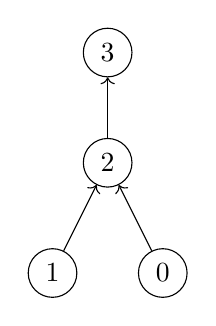
\begin{tikzpicture}
	\node [fill=white, draw=black, shape=circle] (0) at (0.7, -1.4) {0};
	\node [fill=white, draw=black, shape=circle] (1) at (-0.7, -1.4) {1};
	\node [fill=white, draw=black, shape=circle] (2) at (0, 0) {2};
	\node [fill=white, draw=black, shape=circle] (3) at (0, 1.4) {3};
	\draw [fill=none, ->] (0) to (2);
	\draw [fill=none, ->] (1) to (2);
	\draw [fill=none, ->] (2) to (3);
\end{tikzpicture}
\end{minipage}
\begin{minipage}{0.3\textwidth}
\centering
\begin{Verbatim}[frame=single, label=CNF file]
p cnf 7 7
2 1 0
-2 3 0
5 -4 0
-3 0
4 3 0
4 -6 7 0
-4 6 0
\end{Verbatim}
\end{minipage}
\begin{minipage}{0.3\textwidth}
\centering
\begin{Verbatim}[frame=single, label=DAG file]
DAG-FILE
NODES:4
GRAPH:
0->2:1,3
1->2:3,4
2->3:4
CLAUSES:
0:0,1
1:2,3
2:4
3:5,6
REPORTING:
4,6,7
\end{Verbatim}
\end{minipage}

\caption[Hand-worked CNF and DAG file examples]{Example \textsc{Dagster} inputs of a CNF and DAG file. The directed graph described in the DAG file is depicted graphically on the left-hand side.}\label{fig:cnf_dag_example}
\end{figure}




\subsection{An Intuitive View of DAG Decomposition}

To aid understanding, it may be helpful to provide an informal illustration of the kinds of problems and how they might best be related to an appropriate DAG.
The motivation of the \textsc{Dagster} tool was to solve planning-type problems and this is a natural illustration of the kinds of problems which \textsc{Dagster} is designed to solve.

Particularly we might understand a dag structure between nodes $0,1,2,3$ as might be graphed in Figure \ref{fig:cnf_dag_example}.
In this figure, we might consider that nodes $0$ and $1$ are parts of the problem that are naturally solved in parallel and are predominantly independent of each other.
The intersection of their solutions are then passed to node $1$, whose outputs are then passed as constraints to node $2$ whereby we might imagine nodes $1$ and $2$ are problems which are naturally
solved in sequence.

An illustration of the kind of problem that these nodes might correspond is parts of a planning procedure, particularly we might imagine a procedure of travelling to another country being
composed of subtasks which bear relations between them.
We might imagine that nodes $0$ and $1$ relate to the relatively independent subtasks of how to pack your luggage, and problem of choosing modes of transport to the airport.
In this way the problems of nodes $0$ and $1$ relate to subproblems that are relatively independent, in that the way you pack your luggage would (most often) be rather independent of the possible
ways that you could navigate to the airport.
The intersection of solutions to nodes $0$ and $1$ feeds into nodes $2$ which may be the subtask of choosing an airline flight, which would depend on the result of a choice of transport (node $1$) and
be dependent on the way in which the luggage was packed (output from node $0$); perhaps the transport constrains your arrival time at the airport, and the luggage packing constrains your flight by
luggage weight and dimensional restrictions.
Consequently the output of node $2$, informs which flight you can take, and subsequently constrains the solutions of node $3$ which might be the subtask of choosing your in-flight meal.

Although this illustration is simplistic, it illustrates the fact that problems can have a natural structure and how this might correspond to elements of a DAG decomposition of the problem.
%It also illustrates that this structure can be exploited. Particularly it is noticed that solving this problem in the forward direction is most natural and sensible, wheras
%solving it in the reverse direction (or wholistically) is potentially more difficult.

Some general directions are:
\begin{enumerate}
\item	In a sequence it is better for more constrained problems to occur first, in that the output from the more constrained problem should bind the solutions from the less constrained problem
\item	subproblems that are mostly (or entirely) independent should occur in parallel
\item	partitions between the clauses that define the nodes of the problem should correspond with meaningful subproblems - 
which are somewhat difficult (not trivially easy), generate few solutions (as opposed to voluminously many) and naturally constrain further subproblems.
\end{enumerate}


\subsection{Where can I find DAGs?}


There are a range of schemes from the literature which provide recipes for computing a decomposition given the object to be decomposed~\cite{conf/ictai/HabetPT09,NEURIPS2019_6e62a992}.
We also note that lookahead mechanisms, for example as described for cube and conquer approaches to Boolean SAT~\cite{cube_and_conquer1}, provide a decomposition that can be represented using a DAG schematic. 

One class of problem that has always been a focus of this initiative is bounded model checking of safety properties. 
In this setting, a range of literature has already contemplated and described dependency structures between problem variables that can be expressed using a DAG.
%%
In particular we have the concept of a {\em dependency graph}, also sometimes called {\em causal} graph\cite{Knoblock94,WilliamsN97}.
A dependency graph expresses dependencies between problem variables in terms of the ability of one variable to impact the value of another in time -- i.e. in a discrete event system setting.
For some classes of problems such graphs expose small subproblems with few interconnections, with the subproblems’ size independent of parameters determining the overall problem size.
These graphs can be computed quickly (in linear time), and provided exactly the schematic we desire to represent a larger overall problem about a transition system model in terms of a series of abstract subproblems and their refinements.  
A number of ancillary student projects are progressing exactly these ideas, both in a classical planning setting and also in the setting of software/protocol verification. 


\section{Scheduling Process}\label{sec:configuration}

Fundamentally \textsc{Dagster} is a parallel SAT solver, and the compute cores allocated to \textsc{Dagster} are each given a specific role.
Particularly \textsc{Dagster} obeys a Master/Worker dichotomy, where the Master keeps track of the work that needs to be done and allocates appropriate work to the Workers, who
report back to Master the results of their computations.

The first and most natural description of the process occurs from the Master's perspective, particularly the Master coordinates what Workers should be working on what parts of the DAG.
Initially when \textsc{Dagster} begins it sets the workers onto the initial leaf nodes of the DAG (for instance nodes $0$ and $1$ in figure \ref{fig:cnf_dag_example})
and these workers will gradually generate solutions for those nodes, the Master will then record these solutions and from them generate new messages that will be given to workers to
initiate and constrain work on for further nodes (for instance node $2$).
%For each of the further nodes there will need to be run multiple times with slightly different computations depending on the solutions that are passed from the previous nodes.
In this way, solutions to earlier nodes seed computational runs on further nodes, and the Master process coordinates and keeps track of all the work that is yet to be done and has been done.
It does this through a compact representation of the logic of these solutions embedded in Binary Decision Diagrams (BDDs)
particularly using the CUDD library\footnote{see: \url{https://davidkebo.com/cudd}} for BDD manipulation and generation.

\textsc{Dagster} is allowed to run in multiple `modes' identifying the resources which the workers are allocated.
Particularly worker processes are grouped in worker groups, which are given work from Master.
In the simplest operation of \textsc{Dagster}, mode $m=0$, each worker group is a single core running a TiniSAT CDCL process, and when the Master passes a message to the worker process it loads the 
CNF associated with the node it is to work on.
Any solutions generated by the CDCL search are then reported back to Master and serve to seed computation on further nodes.
When the CDCL procedure has finished generating all solutions for a message it then requests further work from the Master process.

In more complicated operational mode $m=1$, each worker group is a single core running a CDCL process and an additional $k$ processes running the SLS gnovelty procedure.
The Master gives the CDCL process the message identifying what node of the DAG it is to be working on and what constraints it is to have, and the CDCL procedure passes the information
to the SLS processes which then initialize and process the problem aswell.
The gnovelty processes give variable suggestions to the CDCL procedure as well as report solutions as they discover them in conjunction to the CDCL procedure.
As before, when the CDCL procedure has verified that all solutions have been generated, it stops the work of the gnovelties and requests further work from the Master.

In a yet more complicated operational mode $m=2$, each worker group is a single running CDCL process, an additional $k$ gnovelty processes and an additional clause strengthener procedure.
As before the Master's message is given to the CDCL procedure, the gnovelties and the strengthener process, and the strengthener process assists the CDCL procedure by strengthening
the conflict clauses that the CDCL procedure generates.

In these three operational modes $m=1,2,3$ each worker group has different numbers of processes in a worker group that is visible to the Master process and which the master interacts with

\begin{enumerate}
\item	Mode zero: each worker group is a single CDCL process (particularly Tinisat)
\item	Mode one: each worker group is composed of a single CDCL process, and $k$ gnovelty processes
\item	Mode two: each worker group is composed of a single CDCL process, assisted by another strengthener process, and $k$ gnovelty processes
\end{enumerate}

An illustration of the elements of the modes are depicted in figure \ref{fig:dagster_organisation}.

The choice of operational mode for \textsc{Dagster} is selected by command line argument, with mode zero as the default.
Additionally, \textsc{Dagster} has command line configuration identifying the way in which the master will coordinate the worker groups.
Particular configuration specifies whether master will preferentially allocate messages that are depth-first in the DAG in an attempt to race to a solution for the problem, 
or alternatively to allocate breadth-first and solve all layers of the DAG structure more systematically.
in this context there is also additional configuration regarding whether \textsc{Dagster} will terminate as soon as it finds a solution to the whole problem, or if it should attempt to generate
all solutions to the problem.
The optimal choice of these options will be expected to depend on the particular problem which \textsc{Dagster} is presented with.


\begin{figure}
\centering     
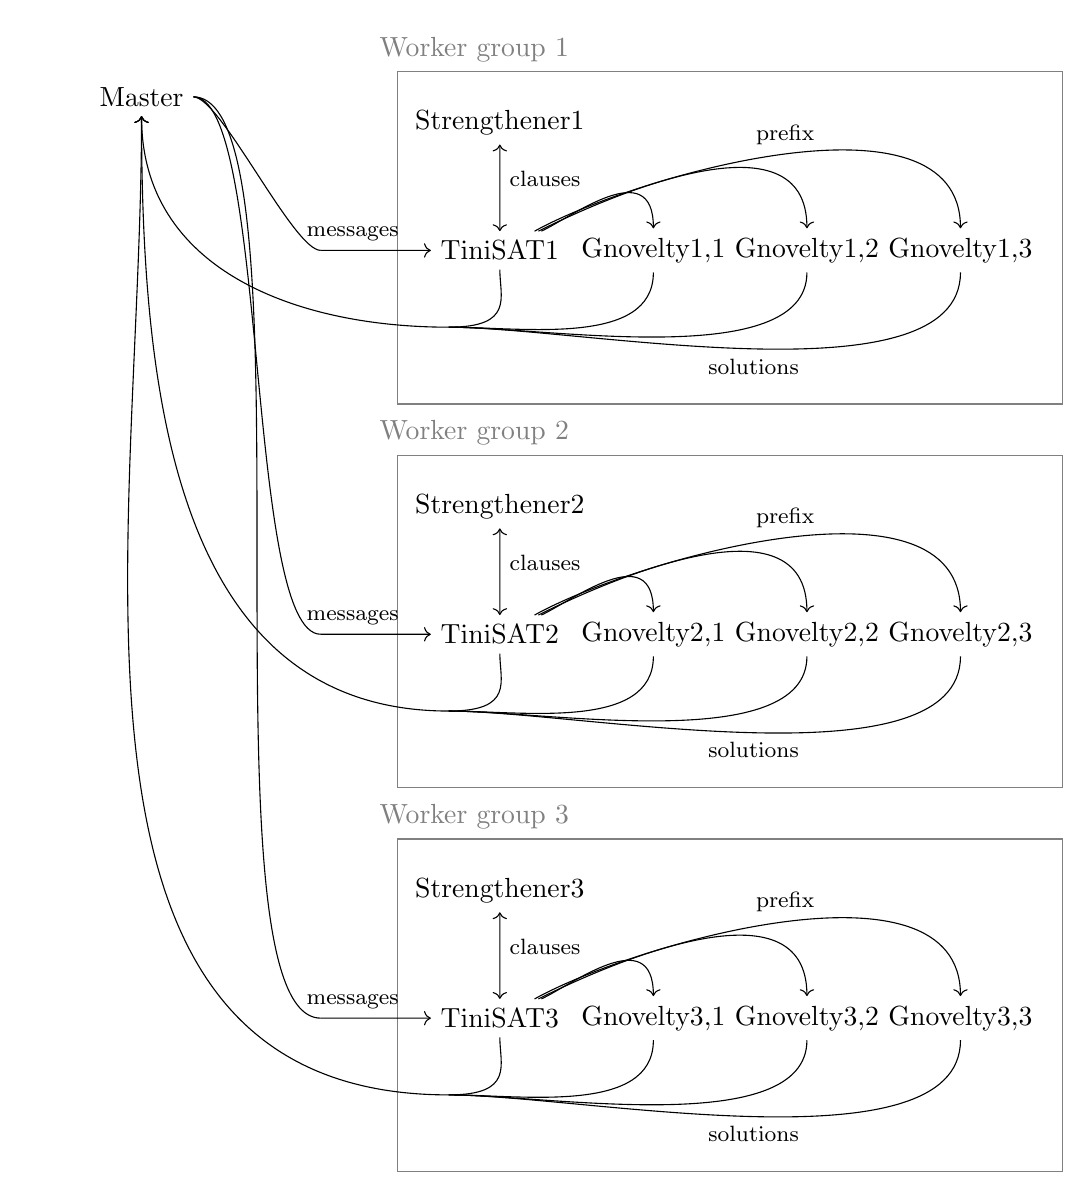
\begin{tikzpicture}[xscale=0.65,yscale=-0.65]

\node (master)	at (-4.0,1.0)	[align=center] {Master};

\node (worker_group_label1)	at (2.5,0.5)	[above,gray] {Worker group 1};
\draw [gray]  (1.0,0.5) -- (14.0,0.5) -- (14.0,7.0) -- (1.0,7.0) -- cycle ;
\node (strengthener1)	at (3.0,1.5)	[align=center] {Strengthener1};
\node (tinisat1)		at (3.0,4.0)	[align=center] {TiniSAT1};
\node (gnovelty11)	at (6.0,4.0)	[align=center] {Gnovelty1,1};
\node (gnovelty12)	at (9.0,4.0)	[align=center] {Gnovelty1,2};
\node (gnovelty13)	at (12.0,4.0)	[align=center] {Gnovelty1,3};
\draw [-,out=0,in=180,looseness=0.35] (master.east) to (-0.5,4.0);
\draw [->,out=0,in=180,looseness=0.75] (-0.5,4.0) to node[above,pos=0.3]{\footnotesize messages} (tinisat1);
\draw [-,out=90,in=0,looseness=1.55] (tinisat1) to (2.0,5.5);
\draw [->,out=180,in=90,looseness=1.05] (2.0,5.5) to  (master.south);
\draw [-,out=90,in=0,looseness=0.90] (gnovelty11.south) to (2.0,5.5);
\draw [-,out=90,in=0,looseness=0.70] (gnovelty12.south) to (2.0,5.5);
\draw [-,out=90,in=0,looseness=0.65] (gnovelty13.south) to node[below,pos=0.5]{\footnotesize solutions} (2.0,5.5);
\draw [->,out=315,in=270,looseness=1.35] (tinisat1) to (gnovelty11.north);
\draw [->,out=320,in=270,looseness=1.05] (tinisat1) to (gnovelty12.north);
\draw [->,out=320,in=270,looseness=0.85] (tinisat1) to node[above,pos=0.5]{\footnotesize prefix} (gnovelty13.north);
\draw [<->,out=270,in=90,looseness=1.55] (tinisat1) to node[right,pos=0.8]{\footnotesize clauses} (strengthener1.south);

\node (worker_group_label2)	at (2.5,8.0)	[above,gray] {Worker group 2};
\draw [gray]  (1.0,8.0) -- (14.0,8.0) -- (14.0,14.5) -- (1.0,14.5) -- cycle ;
\node (strengthener2)	at (3.0,9.0)	[align=center] {Strengthener2};
\node (tinisat2)		at (3.0,11.5)	[align=center] {TiniSAT2};
\node (gnovelty21)	at (6.0,11.5)	[align=center] {Gnovelty2,1};
\node (gnovelty22)	at (9.0,11.5)	[align=center] {Gnovelty2,2};
\node (gnovelty23)	at (12.0,11.5)	[align=center] {Gnovelty2,3};
\draw [-,out=0,in=180,looseness=0.35] (master.east) to (-0.5,11.5);
\draw [->,out=0,in=180,looseness=0.75] (-0.5,11.5) to node[above,pos=0.3]{\footnotesize messages} (tinisat2);
\draw [-,out=90,in=0,looseness=1.55] (tinisat2) to (2.0,13.0);
\draw [->,out=180,in=90,looseness=1.05] (2.0,13.0) to  (master.south);
\draw [-,out=90,in=0,looseness=0.90] (gnovelty21.south) to (2.0,13.0);
\draw [-,out=90,in=0,looseness=0.70] (gnovelty22.south) to (2.0,13.0);
\draw [-,out=90,in=0,looseness=0.65] (gnovelty23.south) to node[below,pos=0.5]{\footnotesize solutions} (2.0,13.0);
\draw [->,out=315,in=270,looseness=1.35] (tinisat2) to (gnovelty21.north);
\draw [->,out=320,in=270,looseness=1.05] (tinisat2) to (gnovelty22.north);
\draw [->,out=320,in=270,looseness=0.85] (tinisat2) to node[above,pos=0.5]{\footnotesize prefix} (gnovelty23.north);
\draw [<->,out=270,in=90,looseness=1.55] (tinisat2) to node[right,pos=0.8]{\footnotesize clauses} (strengthener2.south);

\node (worker_group_label3)	at (2.5,15.5)	[above,gray] {Worker group 3};
\draw [gray]  (1.0,15.5) -- (14.0,15.5) -- (14.0,22.0) -- (1.0,22.0) -- cycle ;
\node (strengthener3)	at (3.0,16.5)	[align=center] {Strengthener3};
\node (tinisat3)		at (3.0,19.0)	[align=center] {TiniSAT3};
\node (gnovelty31)	at (6.0,19.0)	[align=center] {Gnovelty3,1};
\node (gnovelty32)	at (9.0,19.0)	[align=center] {Gnovelty3,2};
\node (gnovelty33)	at (12.0,19.0)	[align=center] {Gnovelty3,3};
\draw [-,out=0,in=180,looseness=0.35] (master.east) to (-0.5,19.0);
\draw [->,out=0,in=180,looseness=0.75] (-0.5,19.0) to node[above,pos=0.3]{\footnotesize messages} (tinisat3);
\draw [-,out=90,in=0,looseness=1.55] (tinisat3) to (2.0,20.5);
\draw [->,out=180,in=90,looseness=1.05] (2.0,20.5) to  (master.south);
\draw [-,out=90,in=0,looseness=0.90] (gnovelty31.south) to (2.0,20.5);
\draw [-,out=90,in=0,looseness=0.70] (gnovelty32.south) to (2.0,20.5);
\draw [-,out=90,in=0,looseness=0.65] (gnovelty33.south) to node[below,pos=0.5]{\footnotesize solutions} (2.0,20.5);
\draw [->,out=315,in=270,looseness=1.35] (tinisat3) to (gnovelty31.north);
\draw [->,out=320,in=270,looseness=1.05] (tinisat3) to (gnovelty32.north);
\draw [->,out=320,in=270,looseness=0.85] (tinisat3) to node[above,pos=0.5]{\footnotesize prefix} (gnovelty33.north);
\draw [<->,out=270,in=90,looseness=1.55] (tinisat3) to node[right,pos=0.8]{\footnotesize clauses} (strengthener3.south);

\end{tikzpicture}
\caption[Messages between components in \textsc{Dagster}]{Relationship and messages between and within the master and worker groups within \textsc{Dagster} mode$2$ operation}\label{fig:dagster_organisation}
\end{figure}


\section{Sources of Decomposed Problems}


There are a range of schemes from the literature which provide recipes for computing a decomposition given the object to be decomposed~\cite{conf/ictai/HabetPT09,NEURIPS2019_6e62a992}.
We also note that lookahead mechanisms, for example as described for cube and conquer approaches to Boolean SAT~\cite{cube_and_conquer1}, provide a decomposition that can be represented using a DAG schematic. 

One class of problem that has always been a focus of this initiative is bounded model checking of safety properties. 
In this setting, a range of literature has already contemplated and described dependency structures between problem variables that can be expressed using a DAG.
%%
In particular we have the concept of a {\em dependency graph}, also sometimes called {\em causal} graph\cite{Knoblock94,WilliamsN97}.
A dependency graph expresses dependencies between problem variables in terms of the ability of one variable to impact the value of another in time -- i.e. in a discrete event system setting.
For some classes of problems such graphs expose small subproblems with few interconnections, with the subproblems’ size independent of parameters determining the overall problem size.
These graphs can be computed quickly (in linear time), and provided exactly the schematic we desire to represent a larger overall problem about a transition system model in terms of a series of abstract subproblems and their refinements.  
A number of ancillary student projects are progressing exactly these ideas, both in a classical planning setting and also in the setting of software/protocol verification. 


\section{Performance Demonstration}

In order to attempt to characterize the \textsc{Dagster} engine, we considered the execution time across a family of stochastically generated problems.
Particularly we considered the generation of random problems reminiscent of \cite{DBLP:journals/jair/JiaMS07}.
In \cite{DBLP:journals/jair/JiaMS07}, random SAT problems are generated by selecting in-advance a satisfying assignment to the problem, and then clauses are constructed within the problem which
always include at-least one literal from the satisfying assignment.
In this way, each additional clause that is added to the problem reduces the space of satisfying solutions, but is guaranteed to preserve the pre-selected satisfying solution; and 
thus the solution of the CNF is guaranteed to be SAT.
The difficulty of the resulting problem is characterized by the total number of variables and the number of clauses added, additionally by how likely each clause is likely to 
have different numbers of literals coincident with the original satisfying assignment.

Taking inspiration from this approach, we constructed a series of these subproblems which each having the same number of variables and clauses, and sharing some variables in common with the one previous.
Thus we were able to generate a family of random structured problems, as given by algorithm \ref{algorithm1}.

\SetKw{KwBy}{by}
\begin{algorithm}[H]
\SetAlgoLined
\KwIn{subproblem variable size $s$, subproblem variable overlap $p$, number of subproblems $n$, clause size $c$, clause multiplier $m$}
\KwOut{a set of clauses of a CNF}
 Consider subproblem $i$ has variable set $V_i=\{(s-p)i+1,\dots,(s-p)i+s\}$\;
 Create a random solution $S = \{\text{Random}(a,\lnot a) : a\in\cup_i V_i\}$\;
 Start with an empty CNF\;
 \For{$i\gets 1$ \KwTo $s$}{
  \For{$j\gets 1$ \KwTo $m$}{
   \For{$v\in V_i$} {
    Construct a subset $H$ of size $c-1$ which does not include $v$, from variables in $V_i$\;
    Construct a clause $C = \{v ~\text{if}~ v\in S ~\text{else}~ \lnot v\}\cup\{\text{Random}(a,\lnot a) : a\in H\}$\;
    Append $C$ to CNF\;
   }
  }
 }
 \caption{Random structured problem construction}\label{algorithm1}
\end{algorithm}

The generated problems naturally have a structure which is amenable to sequential solving, and DAG files were generated to solve each of the subproblems in sequence.
The CNF of all these subproblems together can also directly be passed to traditional SAT solvers for resolution.
In this way the execution time required to solve the subproblems together can be measured by traditional SAT solvers against our \textsc{Dagster} engine.
and the results of some of these runs are shown in figures \ref{fig:performance_graph1} and \ref{fig:performance_graph2}.
In these figures is shown the execution time required for \textsc{Dagster} and \textsc{Minisat} to come to a solution of the generated problems for different clause multiplier $m$ in the generation
procedure per Algorithm \ref{algorithm1}.
The graphs show the median solving time (with a 60s timeout) together with the inter-quartile range (between the first and third quartiles) on the solution times.
Figure \ref{fig:performance_graph1} shows the execution times when the number of overlapping variables between the subproblems is $5$, and Figure \ref{fig:performance_graph2} shows the execution times when the
number of overlapping variables between the subproblems is $15$.

We notice significant differences between the performance of \textsc{Minisat} and \textsc{Dagster} depending on the clause multiplier $m$, particularly that when $m$ is small, all of the
subproblems are markedly under-constrained and it is easy and quick for both \textsc{Minisat} and \textsc{Dagster} to generate a solution to the problem.
However as $m$ increases, and the problems become marginally more constrained, then the performance of \textsc{Dagster} suffers particularly for an interface size of $15$.
This is primarily because an under-constrained problem generates a large number of assignments between the interfaces of the problem (particularly when the interface size is large)
, and when the problem is sufficiently constrained such that most of these are ultimately discarded in the subsequent processing it is unsurprising that \textsc{Dagster} suffers.
However in this region \textsc{Minisat} still has performance, as it tackles the problem holistically, and opportunistically solves particular parts of the problem in an order that suits it.

There is a middle region where both \textsc{Minisat} and \textsc{Dagster} struggle, where $m$ is high enough for the problem to be intractable for \textsc{Minisat}, but not yet over-constrained enough
for \textsc{Dagster} to be advantageous.
And there is a final region of higher $m$ where the subproblems begin to be more constrained, and where solutions of one part of the problem begin to be materially constraining on the solution
to other subproblems, and in this region \textsc{Dagster} has the opportunity to occasionally pull ahead and solve the problem again.
Ultimately in the limit where $m$ is very large, and all subproblems are over-constrained then a solution of one subproblem effectively solves all subsequent subproblems 
(perhaps even by unit-propagation in the extreme case), and in this case \textsc{Dagster} pulls ahead decisively as it solves all subproblems in order, whereas \textsc{Minisat} stalls as it considers all 
subproblems together holistically.

These figures constitute an example of a family of structurally generated random SAT problems in which \textsc{Dagster} has demonstrated performance improvement against \textsc{Minisat}.


%\begin{figure}
%\centering  
%\begin{tikzpicture}[x=0.75pt,y=0.75pt,yscale=-1,xscale=1]
%\draw   (40,40) -- (110,40) -- (110,80) -- (40,80) -- cycle ;
%\draw   (100,50) -- (170,50) -- (170,90) -- (100,90) -- cycle ;
%\draw   (160,60) -- (230,60) -- (230,100) -- (160,100) -- cycle ;
%\draw (75,60) node   [align=center] {SAT1};
%\draw (135,70) node   [align=center] {SAT2};
%\draw (195,80) node   [align=center] {SAT3};
%\draw (255,90) node   [align=center] {...};
%\end{tikzpicture}
%\caption{Relation of random sat generator subproblems}\label{fig:subproblem_construction}
%\end{figure}


   \begin{figure}[h]
        \centering
		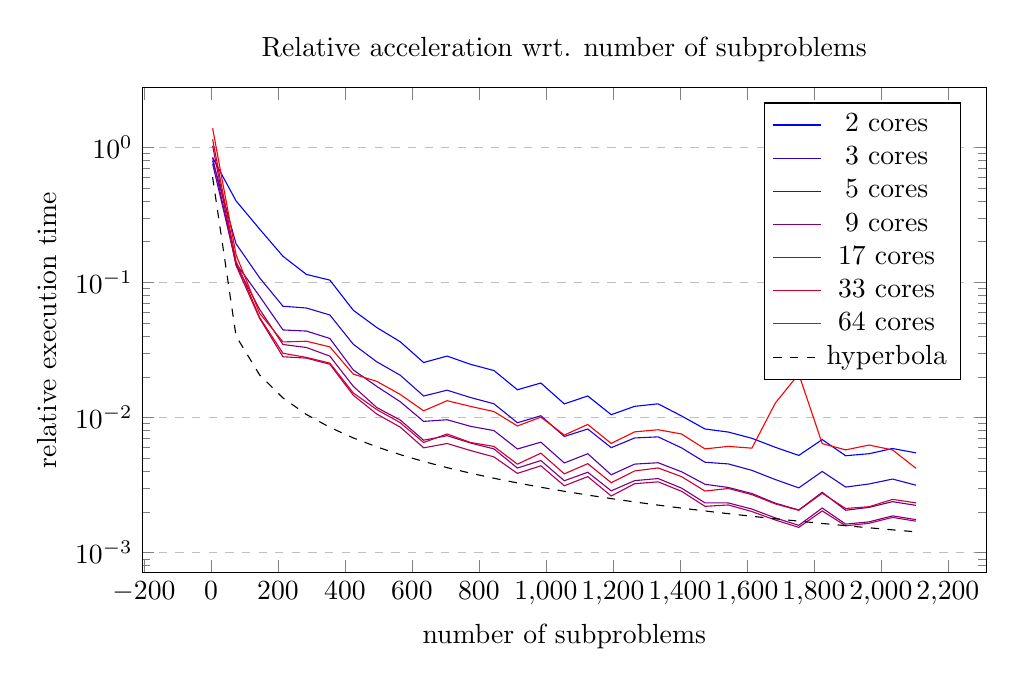
\begin{tikzpicture}
		\begin{axis}[
			title={Relative acceleration wrt. number of subproblems},
			xlabel={number of subproblems},
			ylabel={relative execution time},
			%xmin=0, xmax=0.25,
			%ymin=10.00, ymax=100000.00,
			ymode=log,
			%xmode=log,
			%xtick={0,0.05,0.1,0.15,0.2,0.25},
			%ytick={0,20,40,60,80,100},
			%yticklabel=$\pgfmathprintnumber{\tick}\%$,
			legend pos=north east,
			ymajorgrids=true,
			grid style=dashed,
			xticklabel style={/pgf/number format/fixed},
			width = 350,
			height = 220
		]




\addplot[color=red!0.0!blue,line width=0.4pt] coordinates {
(5,0.8363703260509081)(75,0.40044086669564954)(145,0.24820760445286044)(215,0.15586154433903676)(285,0.11441574489877396)(355,0.10383228199616126)(425,0.062112244462297336)(495,0.04631987498640051)(565,0.0363514389443031)(635,0.0255062395908254)(705,0.028461983857429193)(775,0.024729523125231637)(845,0.02224756104517527)(915,0.016031056959308215)(985,0.017990965806449793)(1055,0.012602624715768295)(1125,0.014428008140009687)(1195,0.010483218052462122)(1265,0.012090345845853636)(1335,0.012617655143597912)(1405,0.010260395984662996)(1475,0.00821915969199854)(1545,0.007797760326512107)(1615,0.007015986107255104)(1685,0.006015559914820198)(1755,0.005238103290395365)(1825,0.006863269191829858)(1895,0.005212129656505115)(1965,0.005394250241223485)(2035,0.005892540631817077)(2105,0.005470470118470802)
}node[pos=0.8](endofplotsquare){} ;
\addlegendentry{2 cores}
\addplot[color=red!16.666666666666668!blue,line width=0.4pt] coordinates {
(5,0.7953947640462143)(75,0.19287219486951168)(145,0.10821465405457484)(215,0.06655933633194881)(285,0.06455734436647677)(355,0.05731206548874832)(425,0.0348103366827173)(495,0.02582226849746521)(565,0.020555985130909643)(635,0.014414085069604093)(705,0.015914041554104696)(775,0.01404563934603624)(845,0.012622724691626362)(915,0.00914084020222177)(985,0.01030137267781949)(1055,0.007236220870675304)(1125,0.008216274992029135)(1195,0.00597728023540709)(1265,0.0070535371403745335)(1335,0.007186896657302999)(1405,0.005957848712307183)(1475,0.004664177373220047)(1545,0.004531664358657725)(1615,0.004062888962836021)(1685,0.003472003348871099)(1755,0.003014331883154194)(1825,0.003989341538922921)(1895,0.0030551923392005942)(1965,0.0032216065883479707)(2035,0.0035026558761778624)(2105,0.00315456432254383)
}node[pos=0.8](endofplotsquare){} ;
\addlegendentry{3 cores}
\addplot[color=red!33.333333333333336!blue,line width=0.4pt] coordinates {
(5,0.7540799612489124)(75,0.13770773845147158)(145,0.07903118735302324)(215,0.0444292876122649)(285,0.04359841132583865)(355,0.03843108751108544)(425,0.022476245693874835)(495,0.016992134208814662)(565,0.013085171580030565)(635,0.009354873212661784)(705,0.009623132156813024)(775,0.008601600810769768)(845,0.007997350837381617)(915,0.005844809497154642)(985,0.006566702190397072)(1055,0.0046066955464967385)(1125,0.005391459880088773)(1195,0.003765944493922464)(1265,0.004517972989232357)(1335,0.004625354886416106)(1405,0.003967271630504892)(1475,0.003204556537457041)(1545,0.003033559290311071)(1615,0.002736811668500518)(1685,0.0023219705479595233)(1755,0.0020689990640417135)(1825,0.0027955377403811573)(1895,0.002059099664076773)(1965,0.002161659972390088)(2035,0.0023835551937098024)(2105,0.0022366735124972883)
}node[pos=0.8](endofplotsquare){} ;
\addlegendentry{5 cores}
\addplot[color=red!50.0!blue,line width=0.4pt] coordinates {
(5,0.8395180080320743)(75,0.13518033229705892)(145,0.06329495573875105)(215,0.03467498095786615)(285,0.032946276058190636)(355,0.02843740849447381)(425,0.01700059475426545)(495,0.01185082078331524)(565,0.009583217651849624)(635,0.0067879373357470785)(705,0.00733279588264961)(775,0.006473730136613454)(845,0.00585275388825431)(915,0.004223941423046687)(985,0.0048023948235786365)(1055,0.0034030299592173706)(1125,0.003932382641530949)(1195,0.0028652830044705252)(1265,0.003409755894449815)(1335,0.003533730715612736)(1405,0.003001564873126131)(1475,0.0023343136294482034)(1545,0.002331287468822943)(1615,0.002099444456355938)(1685,0.0018067291136231742)(1755,0.0015921906675146404)(1825,0.002138097873277723)(1895,0.0016254754718868349)(1965,0.0016898415459182174)(2035,0.0018712422685091005)(2105,0.0017544596847386673)
}node[pos=0.8](endofplotsquare){} ;
\addlegendentry{9 cores}
\addplot[color=red!66.66666666666667!blue,line width=0.4pt] coordinates {
(5,1.0233671083266738)(75,0.13298582581574836)(145,0.054342141287111095)(215,0.028136617662919666)(285,0.0274850117836712)(355,0.024767735467616722)(425,0.014603392440664225)(495,0.01060627134337961)(565,0.008489780577146392)(635,0.005960846427571119)(705,0.006419783187656039)(775,0.005693731627707895)(845,0.005107422343337776)(915,0.003857476739178135)(985,0.004391044049971209)(1055,0.0031239152675193596)(1125,0.0036507550214886614)(1195,0.0026247982449260168)(1265,0.003233826478061956)(1335,0.0033403745852336394)(1405,0.0028430792367325646)(1475,0.002200627944362014)(1545,0.0022523276938355174)(1615,0.002013942986585552)(1685,0.0017432388265270233)(1755,0.0015377756992326164)(1825,0.0020356102833054817)(1895,0.0015788129786271285)(1965,0.0016499736740357815)(2035,0.001822449738409042)(2105,0.0017085385916049166)
}node[pos=0.8](endofplotsquare){} ;
\addlegendentry{17 cores}
\addplot[color=red!83.33333333333333!blue,line width=0.4pt] coordinates {
(5,1.1430591924550146)(75,0.1430227631420044)(145,0.0550902628411104)(215,0.029860641277366737)(285,0.027825714476219225)(355,0.025254507640047268)(425,0.015181667878617168)(495,0.011448534033175722)(565,0.00915695381741731)(635,0.0065301049757312294)(705,0.007550217807928795)(775,0.006531482865975962)(845,0.0061084692678245595)(915,0.004514001544709272)(985,0.005442886204953784)(1055,0.0038276532255329407)(1125,0.004553502202237839)(1195,0.0032922630420942297)(1265,0.004022898124369985)(1335,0.004232557187196659)(1405,0.003650674441859657)(1475,0.002855195221820208)(1545,0.0029828610389978022)(1615,0.002686401608577915)(1685,0.0022927407726168027)(1755,0.0020568970810727625)(1825,0.0027495482073485065)(1895,0.002122191389302815)(1965,0.0021869364529382984)(2035,0.0024771185156596577)(2105,0.002335438636016641)
}node[pos=0.8](endofplotsquare){} ;
\addlegendentry{33 cores}
\addplot[color=red!100.0!blue,line width=0.4pt] coordinates {
(5,1.3804728949138354)(75,0.15989108763659018)(145,0.05923250293374861)(215,0.03623345150554006)(285,0.0366491697816772)(355,0.033302831517728865)(425,0.020934522465703542)(495,0.01850792801621138)(565,0.014818050848156503)(635,0.01120213017824374)(705,0.013307029888745294)(775,0.012078063979757607)(845,0.011056552004666573)(915,0.008652946816065623)(985,0.010058157334588409)(1055,0.007411647218094335)(1125,0.008876128923162509)(1195,0.006425619803304469)(1265,0.007824727583313294)(1335,0.008115708281487758)(1405,0.007548032452182414)(1475,0.005855031785751925)(1545,0.006111780178658547)(1615,0.0059283175789550694)(1685,0.012789253519400294)(1755,0.020957095312401513)(1825,0.0064057552276834415)(1895,0.005760009494321792)(1965,0.006250122294819795)(2035,0.005750178328994417)(2105,0.004205274975490067)
}node[pos=0.8](endofplotsquare){} ;
\addlegendentry{64 cores}
\addplot[color=black,line width=0.4pt,dashed] coordinates {
(5,0.6)(75,0.04)(145,0.020689655172413793)(215,0.013953488372093023)(285,0.010526315789473684)(355,0.008450704225352112)(425,0.007058823529411765)(495,0.006060606060606061)(565,0.005309734513274336)(635,0.004724409448818898)(705,0.00425531914893617)(775,0.003870967741935484)(845,0.0035502958579881655)(915,0.003278688524590164)(985,0.003045685279187817)(1055,0.002843601895734597)(1125,0.0026666666666666666)(1195,0.002510460251046025)(1265,0.0023715415019762848)(1335,0.0022471910112359553)(1405,0.002135231316725979)(1475,0.002033898305084746)(1545,0.001941747572815534)(1615,0.0018575851393188853)(1685,0.0017804154302670622)(1755,0.0017094017094017094)(1825,0.0016438356164383563)(1895,0.0015831134564643799)(1965,0.0015267175572519084)(2035,0.0014742014742014742)(2105,0.0014251781472684087)
}node[pos=0.8](endofplotsquare){} ;
\addlegendentry{hyperbola}

		\end{axis}
		\end{tikzpicture}
		%\vspace{-18pt}
		\caption[Runtime relative acceleration of paralell small-hard problems]{Runtime relative acceleration on paralell small-hard subproblems, relative to Tinisat time, with hyperbolic trendline, for different numbers of cores and subproblems}
		\label{fig:performance_graph1}
    \end{figure}

   \begin{figure}[]
        \centering
		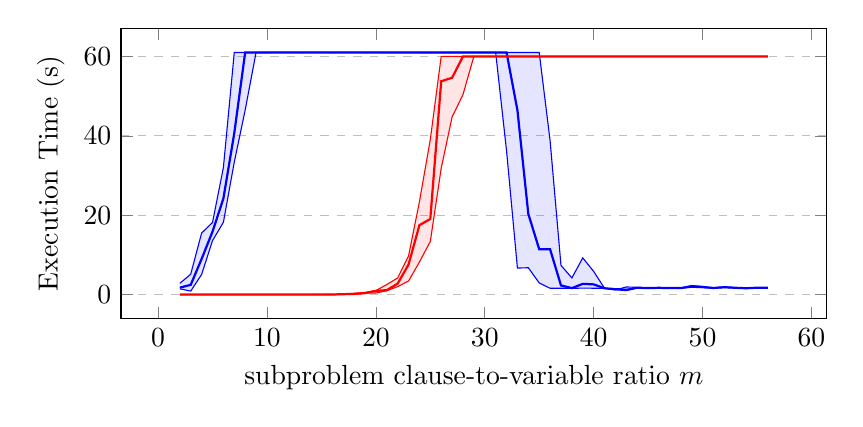
\begin{tikzpicture}
		\begin{axis}[
			title={},
			xlabel={subproblem clause-to-variable ratio $m$},
			ylabel={Execution Time (s)},
			%xmin=0, xmax=0.25,
			%ymin=10.00, ymax=100000.00,
			%ymode=log,
			%xtick={0,0.05,0.1,0.15,0.2,0.25},
			%ytick={0,20,40,60,80,100},
			%yticklabel=$\pgfmathprintnumber{\tick}\%$,
			legend pos=south west,
			ymajorgrids=true,
			grid style=dashed,
			xticklabel style={/pgf/number format/fixed},
			width = 300,
			height = 150
		]



		\addplot[name path=f1,color=blue,line width=0.4pt] coordinates {
(2,1.4639251232147217)(3,0.8906005620956421)(4,5.07472026348114)(5,13.605880618095398)(6,18.212694227695465)(7,33.39086937904358)(8,46.49404948949814)(9,61.00647562742233)(10,61.006454050540924)(11,61.00781857967377)(12,61.00763148069382)(13,61.00721859931946)(14,61.00733244419098)(15,61.00756520032883)(16,61.00716531276703)(17,61.00738650560379)(18,61.00745588541031)(19,61.00723993778229)(20,61.00735676288605)(21,61.00697910785675)(22,61.006991147994995)(23,61.0069962143898)(24,61.006405770778656)(25,61.00641351938248)(26,61.006317019462585)(27,61.00620490312576)(28,61.00618690252304)(29,61.006257236003876)(30,61.00622844696045)(31,61.006043672561646)(32,36.26833963394165)(33,6.685153007507324)(34,6.7725419998168945)(35,2.941969156265259)(36,1.5924944877624512)(37,1.605515480041504)(38,1.582984209060669)(39,1.6359460353851318)(40,1.6101255416870117)(41,1.5897367596626282)(42,1.513471484184265)(43,1.350354731082916)(44,1.6455455422401428)(45,1.6109043955802917)(46,1.6622339487075806)(47,1.6427087783813477)(48,1.6471721529960632)(49,1.8375381827354431)(50,1.7550121545791626)(51,1.6626343131065369)(52,1.7653100490570068)(53,1.697310745716095)(54,1.5819554328918457)(55,1.7184707522392273)(56,1.6828346252441406)
			}node[pos=0.8](endofplotsquare){} ;
		\addplot[color=blue,line width=0.8pt] coordinates {
(2,1.753767967224121)(3,2.4616153240203857)(4,8.982620477676392)(5,15.850266456604004)(6,24.212628841400146)(7,40.69732129573822)(8,61.00638246536255)(9,61.00675821304321)(10,61.00656855106354)(11,61.008005023002625)(12,61.00814092159271)(13,61.00800693035126)(14,61.008145332336426)(15,61.00801944732666)(16,61.007965445518494)(17,61.008007526397705)(18,61.00809359550476)(19,61.00784170627594)(20,61.007810831069946)(21,61.007511496543884)(22,61.00733160972595)(23,61.007174372673035)(24,61.00669300556183)(25,61.007041573524475)(26,61.007081270217896)(27,61.00651478767395)(28,61.00636172294617)(29,61.00694799423218)(30,61.006394386291504)(31,61.006370067596436)(32,61.006324768066406)(33,46.44862389564514)(34,20.325575828552246)(35,11.440356492996216)(36,11.412471055984497)(37,2.3102798461914062)(38,1.6326358318328857)(39,2.710977077484131)(40,2.5742671489715576)(41,1.5958718061447144)(42,1.345030546188354)(43,1.136946082115173)(44,1.735314965248108)(45,1.6483851671218872)(46,1.7121601104736328)(47,1.6433730125427246)(48,1.6472033262252808)(49,2.0652624368667603)(50,1.9037773609161377)(51,1.6716150045394897)(52,1.8630797863006592)(53,1.722955584526062)(54,1.5997889041900635)(55,1.7387510538101196)(56,1.7025666236877441)
			}node[pos=0.8](endofplotsquare){} ;
		\addplot[name path=f2,color=blue,line width=0.4pt] coordinates {
(2,2.8418251276016235)(3,5.140613794326782)(4,15.50329303741455)(5,18.163813292980194)(6,32.00810772180557)(7,61.006208300590515)(8,61.00688475370407)(9,61.00694543123245)(10,61.007078647613525)(11,61.0081524848938)(12,61.00828814506531)(13,61.008241295814514)(14,61.00823652744293)(15,61.00828766822815)(16,61.0080800652504)(17,61.00824177265167)(18,61.0081729888916)(19,61.00811696052551)(20,61.00807774066925)(21,61.00789934396744)(22,61.00771379470825)(23,61.00767105817795)(24,61.00724142789841)(25,61.00723212957382)(26,61.007271349430084)(27,61.00708985328674)(28,61.00680589675903)(29,61.007194340229034)(30,61.00711917877197)(31,61.00664782524109)(32,61.00676250457764)(33,61.006282806396484)(34,61.00626468658447)(35,61.005884885787964)(36,38.782549142837524)(37,7.368508338928223)(38,4.200812101364136)(39,9.258165121078491)(40,5.851057052612305)(41,1.6020068526268005)(42,1.176589608192444)(43,1.92353743314743)(44,1.825084388256073)(45,1.6858659386634827)(46,1.762086272239685)(47,1.6440372467041016)(48,1.6472344994544983)(49,2.2929866909980774)(50,2.052542567253113)(51,1.6805956959724426)(52,1.9608495235443115)(53,1.748600423336029)(54,1.6176223754882812)(55,1.759031355381012)(56,1.7222986221313477)
			}node[pos=0.8](endofplotsquare){} ;
		\addplot[name path=f3,color=red,line width=0.4pt] coordinates {
(2,0.0030400753021240234)(3,0.0032917261123657227)(4,0.0034043192863464355)(5,0.003599405288696289)(6,0.0038619637489318848)(7,0.004148304462432861)(8,0.004418492317199707)(9,0.004787027835845947)(10,0.005482316017150879)(11,0.0058203935623168945)(12,0.006273329257965088)(13,0.007087230682373047)(14,0.007947027683258057)(15,0.010774374008178711)(16,0.019990086555480957)(17,0.04747474193572998)(18,0.1329626441001892)(19,0.34509122371673584)(20,0.40472412109375)(21,0.9638146162033081)(22,2.018075466156006)(23,3.4091747999191284)(24,8.207813739776611)(25,13.376740038394928)(26,31.823628962039948)(27,44.72826838493347)(28,50.38537156581879)(29,60.0020449757576)(30,60.00200414657593)(31,60.0020637512207)(32,60.00204086303711)(33,60.00199103355408)(34,60.00203347206116)(35,60.0020055770874)(36,60.00201463699341)(37,60.002042055130005)(38,60.00200366973877)(39,60.00199270248413)(40,60.002031326293945)(41,60.00443357229233)(42,60.00221532583237)(43,60.00194776058197)(44,60.001987516880035)(45,60.00195640325546)(46,60.00198417901993)(47,60.00202536582947)(48,60.002818524837494)(49,60.00282263755798)(50,60.00277543067932)(51,60.00198030471802)(52,60.00368791818619)(53,60.002643406391144)(54,60.00286382436752)(55,60.00284826755524)(56,60.002190709114075)
			}node[pos=0.8](endofplotsquare){} ;
		\addplot[color=red,line width=0.8pt] coordinates {
(2,0.0034666061401367188)(3,0.003747224807739258)(4,0.003755807876586914)(5,0.0041468143463134766)(6,0.003888845443725586)(7,0.004182219505310059)(8,0.0044689178466796875)(9,0.004850625991821289)(10,0.005688905715942383)(11,0.005968570709228516)(12,0.00668942928314209)(13,0.0075370073318481445)(14,0.009754061698913574)(15,0.015580058097839355)(16,0.024063587188720703)(17,0.10906064510345459)(18,0.17302286624908447)(19,0.37277162075042725)(20,0.9325069189071655)(21,1.1255042552947998)(22,2.7599854469299316)(23,7.56352972984314)(24,17.492953658103943)(25,19.06186842918396)(26,53.74787080287933)(27,54.630271315574646)(28,60.002238273620605)(29,60.002142906188965)(30,60.002079486846924)(31,60.002121448516846)(32,60.00217914581299)(33,60.00208854675293)(34,60.002084732055664)(35,60.002097845077515)(36,60.00210762023926)(37,60.002140283584595)(38,60.003228187561035)(39,60.00205206871033)(40,60.0021538734436)(41,60.00449788570404)(42,60.00223195552826)(43,60.00199794769287)(44,60.00199997425079)(45,60.00196993350983)(46,60.002057671546936)(47,60.00208830833435)(48,60.00339639186859)(49,60.00346493721008)(50,60.00344109535217)(51,60.001983642578125)(52,60.00416123867035)(53,60.00331699848175)(54,60.00343215465546)(55,60.003549575805664)(56,60.00224542617798)
			}node[pos=0.8](endofplotsquare){} ;
		\addplot[name path=f4,color=red,line width=0.4pt] coordinates {
(2,0.003825664520263672)(3,0.008589506149291992)(4,0.004202425479888916)(5,0.004277288913726807)(6,0.004484951496124268)(7,0.004585385322570801)(8,0.004722118377685547)(9,0.004995107650756836)(10,0.005788087844848633)(11,0.006118476390838623)(12,0.007335841655731201)(13,0.008275866508483887)(14,0.011214911937713623)(15,0.03845345973968506)(16,0.03921103477478027)(17,0.14982205629348755)(18,0.3389686942100525)(19,0.5464287400245667)(20,1.021698772907257)(21,2.519692838191986)(22,4.187283217906952)(23,9.699017345905304)(24,23.385829150676727)(25,39.054049134254456)(26,60.00237226486206)(27,60.002327263355255)(28,60.00232529640198)(29,60.0021978020668)(30,60.002198219299316)(31,60.002275466918945)(32,60.00235152244568)(33,60.002241134643555)(34,60.00225043296814)(35,60.00225782394409)(36,60.00218939781189)(37,60.0033004283905)(38,60.00433039665222)(39,60.00389003753662)(40,60.00227689743042)(41,60.00456219911575)(42,60.00224858522415)(43,60.00204813480377)(44,60.00201243162155)(45,60.00198346376419)(46,60.002131164073944)(47,60.00215125083923)(48,60.00397425889969)(49,60.00410723686218)(50,60.004106760025024)(51,60.00198698043823)(52,60.00463455915451)(53,60.00399059057236)(54,60.00400048494339)(55,60.00425088405609)(56,60.00230014324188)
			}node[pos=0.8](endofplotsquare){} ;



\addplot [
        thick,
        color=blue,
        fill=blue, 
        fill opacity=0.1
    ]
    fill between[
        of=f1 and f2
    ];
\addplot [
        thick,
        color=red,
        fill=red, 
        fill opacity=0.1
    ]
    fill between[
        of=f3 and f4
    ];

		\end{axis}
		\end{tikzpicture}
		%\vspace{-18pt}
		\caption[Runtime performance for random structured problems with many overlapping variables]{Runtime performance (medians and interquartile ranges) of \textsc{Dagster} (as blue) and \textsc{Minisat} (as red) for structured problems given by algorithm \ref{algorithm1} with many overlapping variables ($s=100,p=15,s=4,c=5$)}
		\label{fig:performance_graph2}
    \end{figure}




\section{Conclusion and Future Work}


We have presented \textsc{Dagster}, a Boolean SAT solving tool that can distribute and schedule search activities in HPC environments according to a given problem decomposition.
The focus of our activities moving forward is to exploit this tool in a range of settings.
Working collaboratively with students who have already begun their ancillary projects, we will be developing a test suite and evaluation of this approach in the setting of bounded model checking of safety properties, and in particular such problems as they occur in software verification and protocol analysis settings. 
We will be exploring decompositions of structured (from industry and applications) SAT benchmarks according to published schemes, and examining the effectiveness of those in our setting. 



\renewcommand{\refname}{\spacedlowsmallcaps{References}} % For modifying the bibliography heading
\bibliographystyle{unsrt}
\bibliography{bib.bib} % The file containing the bibliography
\end{document}
